\documentclass[11pt]{article}
\usepackage[utf8]{inputenc}
\usepackage[spanish]{babel}
\decimalpoint
\usepackage{amsmath}
\usepackage{amsthm}
\usepackage{amssymb}
\usepackage{graphicx}
\usepackage[margin=0.8in]{geometry}
\usepackage{fancyhdr}
\usepackage[inline]{enumitem}
\usepackage{float}
\usepackage{cancel}
\usepackage{bigints}
\usepackage{listings}
\usepackage{xcolor}
\usepackage{listingsutf8}
\usepackage{algpseudocode}
\usepackage{algorithm}
\usepackage{apacite}
\usepackage{tcolorbox}
\usepackage{multicol}
\usepackage{tipa}
\usepackage{caption} 
\pagestyle{fancy}
\usepackage{hyperref}
\usepackage{mathtools}% http://ctan.org/pkg/mathtools
\hypersetup{
    colorlinks,
    citecolor=black,
    filecolor=black,
    linkcolor=black,
    urlcolor=black
}
\newcommand{\xvdash}[1]{%
	\vdash^{\mkern-10mu\scriptscriptstyle\rule[-.9ex]{0pt}{0pt}#1}%
}
\setlength{\headheight}{15pt} 
\lhead{Atractores y Expresiones Regulares para la regla 22 y 54}
\rhead{\thepage}
\lfoot{ESCOM-IPN}
\renewcommand{\footrulewidth}{0.5pt}
\setlength{\parskip}{0.5em}
\newcommand{\ve}[1]{\overrightarrow{#1}}
\newcommand{\abs}[1]{\left\lvert #1 \right\lvert}
\newcommand{\blank}{\text{\textcrb}}
\date{\today}
\title{Reporte Final.- Atractores y Expresiones Regulares para la regla 22 y 54}
\author{Sanchez Mendez Edmundo Josue}

\lstdefinestyle{customc}{
	belowcaptionskip=1\baselineskip,
	breaklines=true,
	frame=L,
	xleftmargin=\parindent,
	language=C++,
	showstringspaces=false,
	basicstyle=\ttfamily,
	keywordstyle=\bfseries\color{green!40!black},
	commentstyle=\itshape\color{purple!40!black},
	identifierstyle=\color{blue},
	numbers=left,
	stringstyle=\color{orange},
}

\lstset{escapechar=@,style=customc,tabsize=3,language=C++}

\bibliographystyle{apacite}
\begin{document}
		\begin{titlepage}
			\begin{center}
				
				% Upper part of the page. The '~' is needed because \\
				% only works if a paragraph has started.
				
				\noindent
				\begin{minipage}{0.5\textwidth}
					\begin{flushleft} \large
						
\includegraphics[width=0.5\textwidth]{resources/ipn.png}
					\end{flushleft}
				\end{minipage}%
				\begin{minipage}{0.55\textwidth}
					\begin{flushright} \large
						
\includegraphics[width=0.5\textwidth]{resources/escom.png}
					\end{flushright}
				\end{minipage}
				
				\textsc{\LARGE Instituto Politécnico Nacional}\\[0.5cm]
				
				\textsc{\Large Escuela Superior de Cómputo}\\[1cm]
				
				% Title
				
				{ \huge Reporte Final.- Atractores y Expresiones Regulares para la regla 22 y 54  \\[1cm] }
				
				{ \Large Unidad de aprendizaje: Computing Selected Topics} \\[1cm]
				
				{ \Large Grupo: 3CM19 } \\[1cm]
				
				\noindent
				\begin{minipage}{0.5\textwidth}
					\begin{flushleft} \large
						\emph{Alumno:} \\
						Sanchez Mendez Edmundo Josue
					\end{flushleft}
				\end{minipage}%
				\begin{minipage}{0.5\textwidth}
					\begin{flushright} \large
						\emph{Profesor:} \\
						Juarez Martinez Genaro
					\end{flushright}
				\end{minipage}
				
				\vfill
				% Bottom of the page
				{\large {\today}}
			\end{center}
		\end{titlepage}
	
	\titlepage
	\tableofcontents
	\newpage
	
		\begin{abstract}
		Para este reporte abarcaremos la generación de atractores y generación de cadenas aleatorias con base en las expresiones regulares para los autómatas celulares elementales con regla 22 y 54. Nuestro objetivo es poder examinar el comportamiento de estas reglas con base en sus atractores y expresiones regulares, como en el siguiente ejemplo.
	\begin{figure}[H]
			\centering
			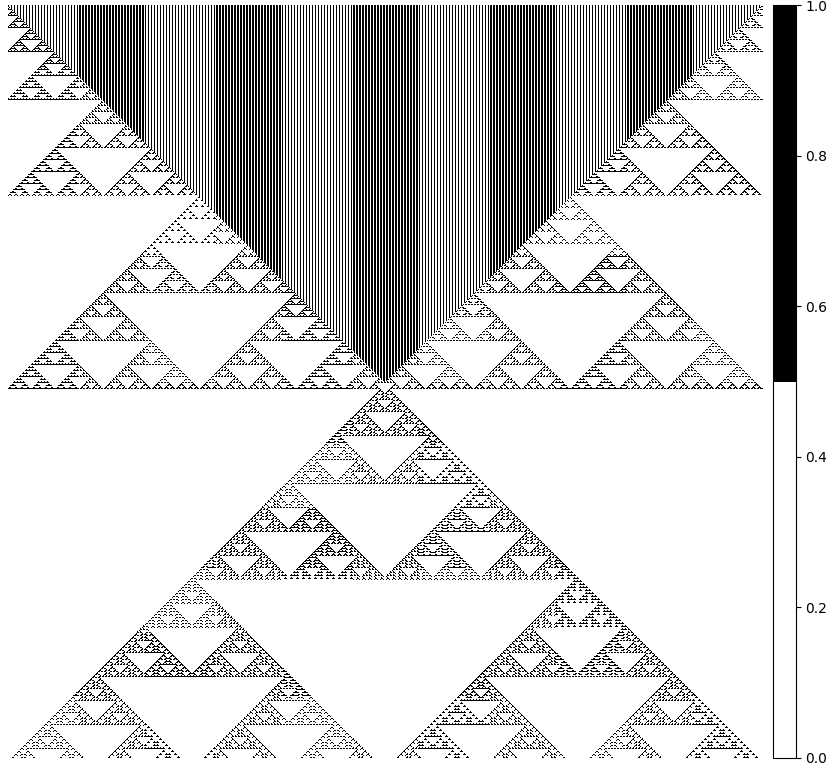
\includegraphics[scale=0.7]{resources/automata_1000x1000_r22.png}
			\caption{Autómata celular elemental de 1000 células evolucionado 1000 veces, regla 22 usando su expresión regular.}\label{fig:picture}
		\end{figure}
	\end{abstract}		
	
	\newpage
	
	\section{Introducción}
		\subsection{Atractores}
		Los atractores son un conjunto de valores numéricos hacia los cuales un sistema tiende a evolucionar, dada por una variedad de condiciones iniciales en el sistema, existen tres tipos de atractores que son los siguientes:
		 \begin{itemize}
    		 \item Atractor de punto fijo: El sistema que tenga un atractor de punto fijo tenderá a estabilizarse en un único punto.
		    \item Atractor de ciclo límite o atractor periódico: Este tipo de atractor tiende a mantenerse en un periodo o en un mismo ciclo.
		    \item Atractor caótico: Aparece en sistemas no lineales que tienen una gran sensibilidad a las condiciones. Un famoso ejemplo de estos atractores es el atractor de Lorenz.
		\end{itemize}\par
		\subsection{Expresiones regulares}		
		Las expresiones regulares nos permiten describir el lenguaje aceptado por un autómata finito, en nuestro caso buscamos ver como el uso de la expresiones regulares que describen a nuestras reglas afectan a la generación de autómatas celulares cuando se usan como condición inicial.
		\subsection{Entropia de Shannon}
		La entropía de Shannon es una de las métricas más importantes en la teoría de la información. La entropía mide la incertidumbre asociada con una variable aleatoria, es decir, el valor esperado de la información en el mensaje (en informática clásica se mide en bits).\par
El concepto fue introducido por Claude E. Shannon en el artículo ``A Mathematical Theory of Communication'' (1948). La entropía de Shannon permite estimar el número mínimo promedio de bits necesarios para codificar una cadena de símbolos en función del tamaño del alfabeto y la frecuencia de los símbolos y viene dada por la siguiente formula:
  \[ H(X) = -\sum_{i=1}^{n} P(x_i)\log_bP(x_i)\]
  En donde b es la base del logaritmo utilizado. Los valores comunes de b son 2, el número de Euler e y 10, y las unidades correspondientes de entropía son los bits para b = 2 , nats para b = e y bans para b = 10 y $P(x_i)$ como la probabilidad de un evento, para nuestro caso de estudio b=2.\par
La situación de máxima incertidumbre nos genera que sea más difícil predecir el resultado siguiente, esto es debido a que hay probabilidad uniforme. La entropía, entonces, solo puede disminuir a partir del valor asociado con la probabilidad uniforme. El caso extremo es donde un estado tiene probabilidad de 1 ya que ahí no hay incertidumbre, es decir la entropía es cero.
	\section{Expresiones Regulares}
		\subsection{Regla 22}
		La expresión regular que nos describe a la regla 22 es el siguiente:\[(0+1(01)^\ast00)(0+0(01)^\ast00)^\ast\]\par
		La expresión regular anterior nos permite poder generar cadenas aleatorias que nos servirán como condiciones iniciales para la generación de nuestros autómatas celulares elementales. Para poder visualizar como el uso de nuestra expresión regular afecta al comportamiento de nuestro autómata haremos las siguientes pruebas:
		\begin{itemize}
    		 \item Probabilidad del 50\% de unos. 
		    \item Probabilidad del 95\% de unos.
		    \item Generación de condición inicial completamente aleatoria.
		\end{itemize}\par
		Estas serán comparadas con cadenas aleatorias generadas mediante la expresión regular, todo esto se hará en un espacio de 400x400 células y se compararan tanto la imagen que nos genera el autómata así como con diferentes métricas que el programa nos proporciona.
		\subsubsection{Probabilidad del 50\% de unos}
		En la figura 2 podemos ver los valores de entrada en nuestro programa, en donde definimos un espacio de 400 x 400 células con una probabilidad de unos del 50\%		
		\begin{figure}[H]
			\centering
			\includegraphics[scale=0.5]{resources/RegEx22/50_prob_entrada.png}
			\caption{Entrada de nuestro programa para la primera prueba.}\label{fig:picture}
		\end{figure}
		En la figura 3 vemos el autómata resultante así como las métricas que el programa nos genera.
		\begin{figure}[H]
			\includegraphics[scale=0.26]{resources/RegEx22/50_prob_result.png}
			\caption{Autómata resultante con sus respectivas métricas.}\label{fig:picture}
		\end{figure}		
		En la figura 4 de igual manera que con la figura 2 podemos ver los valores de entrada de nuestro programa, en donde lo único que cambia es que en esta ocasión hacemos uso de la expresión regular de nuestra regla media la selección de la casilla con la etiqueta ``Use regular expression (rule 22 \& 54 only)''
		\begin{figure}[H]
			\centering
			\includegraphics[scale=0.5]{resources/RegEx22/50_prob_regex_entrada.png}
			\caption{Entrada de nuestro usando nuestra expresión regular r22.}\label{fig:picture}
		\end{figure}
		En la figura 5 vemos el autómata resultante así como las métricas que el programa nos genera.
		\begin{figure}[H]
			\includegraphics[scale=0.26]{resources/RegEx22/50_prob_regex_result.png}
			\caption{Autómata resultante con sus respectivas métricas.}\label{fig:picture}
		\end{figure}
		Antes de empezar con el estudio de estos dos autómatas recordar que la expresión regular se utiliza para poder generar condiciones iniciales aleatorias en las cuales tenemos un control hasta cierto punto, por lo que el autómata mostrado en la figura 5 puede variar en forma y en consecuencia en sus métricas si los comparamos con los autómatas que se generaran en las dos pruebas restantes, una vez mencionado lo anterior, comparemos los resultados.\par
		 Para nuestro autómata con probabilidad del 50\% de unos en la condición inicial vemos como 5 de nuestras 6 gráficas tienen una silueta muy similar entra ellas, vemos como el numero de unos por paso se mantienen entre los valores de 160 y 120 en donde ocasionalmente hay pasos en donde se salen de esos valores,pero nunca llegan a superar a la primera iteración en donde el numero de pasos fue de un poco mas de 200, si vemos la entropia de Shannon vemos que el valor mas alto fue de 1 y el mas bajo de 0.825 esto nos quiere decir que tenemos casi una probabilidad uniforme, esto lo podemos afirmar ya que para poder obtener el valor máximo de la entropia de shannon necesitamos probabilidades iguales, de forma general podemos decir que tenemos una gran incertidumbre y nos vemos incapaces de poder predecir el próximo estado que tomara nuestro autómata, examinando nuestra gráfica de la densidad en la columna central vemos como nos recuerda a una linea recta, es decir su crecimiento es lineal, aunque hay ciertos puntos en donde la densidad fue constante y no tenemos un patrón reconocible en nuestro autómata.\par
		 Por otro lado tenemos al autómata generado por expresión regular y a simple viste podemos observar que es un caso completamente diferente al primero ya que podemos observar cierto patrón en nuestro autómata, el cual pareciese ser la formación de un triangulo isósceles de cabeza y a sus lados patrones formados de triángulos incrustados dentro de un triangulo superior que pareciese que avanzan hasta un punto de unión formando un triangulo diferente. Observado las métricas que tenemos disponibles podemos afirmar que hay un patrón en nuestro autómata ya que las mediciones parecen repetirse por determinados ciclos, podemos ver como el numero de unos va disminuyendo a como pasan las iteraciones y por ello vemos como la densidad de la columna central llega a un máximo de 265 células con valor 1 para pasar a ser constante, vemos a la entropia iniciar con el máximo valor que puede tomar en nuestro caso de estudio a tocar el valor mas bajo, esto quiere decir que en nuestro sistema pasamos de ser incapaces de predecir el siguiente estado a poder predecir el siguiente estado de nuestro autómata.\par
		 En resumen vemos como la expresión regular en este caso nos genera un patrón muy claro en nuestro autómata y como esto influye tanto en la generación de nuestro autómata como en sus métricas en especial caso podemos ver como la entropia de nuestros dos casos de estudio son muy distintos ya que pasamos de tener una entropia casi máxima a tener una entropia casi mínima, es decir pasamos de tener una gran incertidumbre a prácticamente no tener incertidumbre.
		\subsubsection{Probabilidad del 95\% de unos}
		En la figura 6 podemos ver los valores de entrada en nuestro programa, en donde definimos un espacio de 400 x 400 células con una probabilidad de unos del 95\%		
		\begin{figure}[H]
			\centering
			\includegraphics[scale=0.5]{resources/RegEx22/95_prob_entrada.png}
			\caption{Entrada de nuestro programa para la segunda prueba.}\label{fig:picture}
		\end{figure}
		En la figura 7 vemos el autómata resultante así como las métricas que el programa nos genera.
		\begin{figure}[H]
			\includegraphics[scale=0.26]{resources/RegEx22/95_prob_result.png}
			\caption{Autómata resultante con sus respectivas métricas.}\label{fig:picture}
		\end{figure}		
		En la figura 8 de igual manera que con la figura 6 podemos ver los valores de entrada de nuestro programa, en donde lo único que cambia es que en esta ocasión hacemos uso de la expresión regular de nuestra regla media la selección de la casilla con la etiqueta ``Use regular expression (rule 22 \& 54 only)''
		\begin{figure}[H]
			\centering
			\includegraphics[scale=0.5]{resources/RegEx22/50_prob_regex_entrada.png}
			\caption{Entrada de nuestro usando nuestra expresión regular r22.}\label{fig:picture}
		\end{figure}
		En la figura 9 vemos el autómata resultante así como las métricas que el programa nos genera.
		\begin{figure}[H]
			\includegraphics[scale=0.26]{resources/RegEx22/95_prob_regex_result.png}
			\caption{Autómata resultante con sus respectivas métricas.}\label{fig:picture}
		\end{figure}
		 Para nuestro autómata con probabilidad del 95\% de unos en la condición inicial vemos como el numero de unos, el $\log_{10}$ y el valor esperado tienen una silueta muy similar entra ellas de igual forma la varianza con la entropia de Shannon, vemos como el numero de unos por paso tiene un máximo al inicio con un valor de 377 a tener un bajo en la primera iteración teniendo como valor de 9, después de este máximo y mínimo los unos tienden a crecer de una forma logarítmica ya que parece tener una asíntota horizontal en el valor 150, si vemos la entropia de Shannon podemos ver de manera clara como al inicio tenemos el valor mínimo de entropia, es decir no tenemos incertidumbre es prácticamente nula, sin embargo, con el paso de las iteraciones esta incertidumbre va aumentando hasta llegar prácticamente al punto máximo de entropia, es decir tenemos una gran incertidumbre y nos vemos incapaces de poder predecir el próximo estado que tomara nuestro autómata, examinando nuestra gráfica de la densidad en la columna central vemos como es constante el numero de 1's hasta la iteración 58 ya que desde la siguiente iteración comienza a ver un crecimiento escalonado, finalizando el análisis de este autómata podemos decir que no tenemos un patrón reconocible, sin embargo, podríamos decir que al inicio teníamos formas triangulares inscritas en un triangulo mayor pero en un punto estas figuras se perdieron.\par
		 Por otro lado tenemos al autómata generado por expresión regular y a simple viste podemos observar como comparte un patrón con el autómata de la figura 5 y es que vemos como en una parte del autómata tenemos lineas rectas que nos forman un triangulo invertido y vemos como las gráficas no se parecen en nada a la prueba de 95\% de unos. Observado las métricas que tenemos disponibles observamos una gran variación en la información que nos da el autómata y es algo completamente diferente a la prueba que estudiamos ya que en esa prueba vemos como tienden a un valor, en cambio, en este autómata podemos ver como el numero de unos va disminuyendo a como pasan las iteraciones pero no es una disminución constante si no que es como saltado y no es una reducción continua, sin embargo, vemos como la densidad de la columna central va aumentando de una forma casi lineal, pero volvemos a ver como hay puntos en donde el valor no cambia pero en su mayoría son lapsos muy pequeños, pero en la entropia podemos ver como inicia prácticamente en el máximo valor que puede tomar y después de 16 iteraciones empieza a disminuir y oscilar entre los valores 0.8 y 0.975, esto quiere decir que en nuestro sistema dentro de todas las iteraciones nos vemos incapaces de predecir el siguiente estado nuestro autómata y tenemos una alta incertidumbre.\par
		 En resumen vemos como la expresión regular en este caso no nos genera un patrón muy claro en este autómata, sin embargo, vemos como comparte un pequeño patrón con el autómata de la figura 5, asi vemos como la expresión regular sigue influyendo en la generación de nuestro autómata. En esta ocasión volvemos a ver como las métricas no coinciden, sin embargo, podemos ver como hay partes de nuestro autómata que se parecen un poco pero que nos proporcionan información distinta.\newpage
		\subsubsection{Generación de condición inicial completamente aleatoria}
		En la figura 10 podemos ver los valores de entrada en nuestro programa, en donde definimos un espacio de 400 x 400 células haciendo uso de la función random de la librería numpy de Python el cual nos generara un arreglo de determinado tamaño, en este caso de 400 células, lleno aleatoriamente de números 0 y 1.		
		\begin{figure}[H]
			\centering
			\includegraphics[scale=0.5]{resources/RegEx22/random_entrada.png}
			\caption{Entrada de nuestro programa para la tercera prueba.}\label{fig:picture}
		\end{figure}
		En la figura 11 vemos el autómata resultante así como las métricas que el programa nos genera.
		\begin{figure}[H]
			\includegraphics[scale=0.26]{resources/RegEx22/random_result.png}
			\caption{Autómata resultante con sus respectivas métricas.}\label{fig:picture}
		\end{figure}		
		En la figura 12 de igual manera que con la figura 10 podemos ver los valores de entrada de nuestro programa, en donde lo único que cambia es que en esta ocasión hacemos uso de la expresión regular de nuestra regla media la selección de la casilla con la etiqueta ``Use regular expression (rule 22 \& 54 only)''
		\begin{figure}[H]
			\centering
			\includegraphics[scale=0.5]{resources/RegEx22/50_prob_regex_entrada.png}
			\caption{Entrada de nuestro usando nuestra expresión regular r22.}\label{fig:picture}
		\end{figure}
		En la figura 13 vemos el autómata resultante así como las métricas que el programa nos genera.
		\begin{figure}[H]
			\includegraphics[scale=0.26]{resources/RegEx22/random_regex_result.png}
			\caption{Autómata resultante con sus respectivas métricas.}\label{fig:picture}
		\end{figure}
		 Para nuestro autómata generado de manera aleatoria vemos como las gráficas comparten una silueta muy similar entra, vemos como el numero de unos por paso tiene un máximo al inicio con un valor de 200 para después disminuir y rondar valores de 104 como el mas bajo a 182 como el valor mas alto, si vemos la entropia de Shannon podemos ver que volvemos a tener un patrón similar a las pruebas pasadas, en donde comenzamos con prácticamente la entropia máxima a disminuir un poco y oscilar entre los valores 0.825 y 0.9941, esto nos vuelve a indicar que tenemos incertidumbre, examinando nuestra gráfica de la densidad en la columna central vemos un crecimiento prácticamente lineal en el numero de 1's pero hay que mencionar que volvemos a ver partes en donde la gráfica de densidad es constante, finalizando el análisis de este autómata podemos decir que no tenemos un patrón reconocible a diferencia de pruebas pasadas en donde si podríamos llegar a visualizar patrones.\par
		 Por otro lado tenemos al autómata generado por expresión regular y a simple viste podemos observar como volvemos a compartir el patrón de triangulo invertido formado por lineas rectas de valores 0 y 1 intercaladas de los autómatas generados por expresión regular de las pruebas anteriores y de hecho podemos ver un gran parecido con el autómata de la figura 9 tanto en las gráficas como en el mismo autómata solo que el autómata que estamos estudiando tenemos el patrón de los triángulos incrustados en otro aún mayor pero en esta ocasión podemos ver esa patrón mas veces pero volvemos a llegar un punto en donde los  patrones desaparecen. Observado las métricas que tenemos disponibles observamos como el numero de unos tiene un máximo de 382 unos a tener un mínimo de 177 para después empezar a rondar los valores de 211 a 300 células con valor 1, sin embargo, vemos como la densidad de la columna central al inicio tienen un crecimiento lineal entre la iteración inicial hasta la 25 para después volverse constante hasta la iteración 60 en donde ya empieza a existir un incremento casi lineal pero volvemos a ver como hay partes en done es constante, pero en la entropia podemos ver que es muy similar a la vista en la figura 9 en donde vemos como inicia prácticamente en el máximo valor que puede tomar y después de 16 iteraciones empieza a disminuir y oscilar entre los valores 0.79 y 0.99, esto quiere decir que en nuestro sistema dentro de todas las iteraciones nos vemos incapaces de predecir el siguiente estado nuestro autómata y tenemos una alta incertidumbre.\par
		 Una vez visto estas tres pruebas podemos decir que la expresión regular nos genera patrones comunes entre los diferentes autómatas aun a pesar de que esta se genera de manera aleatoria, el patrón mas reconocible son las intercalaciones de columnas de ceros y unos que forman un triangulo invertido, mientras que también existe otro patrón en donde hay triángulos inscritos en un uno mayor y es común ver estos patrones juntos, también vemos como si usamos el 50\%, 95\% e inclusive la formación aleatoria nos generan autómatas en donde la mayor parte de la iteraciones tenemos una gran entropia aunque esto también lo podemos ver en la generada mediante la expresión regular aunque existen formaciones como la figura 5 en donde la entropia llega casi al mínimo valor.
		\subsection{Regla 54}
		La expresión regular que nos describe a la regla 54 es el siguiente: \[(0+1(11)^\ast10)(0+0(11)^\ast10)^\ast\]\par
		La expresión regular anterior nos permite poder generar cadenas aleatorias que nos servirán como condiciones iniciales para la generación de nuestros autómatas celulares elementales. Para poder visualizar como el uso de nuestra expresión regular afecta al comportamiento de nuestro autómata haremos las siguientes pruebas:
		\begin{itemize}
    		 \item Probabilidad del 50\% de unos. 
		    \item Probabilidad del 95\% de unos.
		    \item Generación de condición inicial completamente aleatoria.
		\end{itemize}\par
		Estas serán comparadas con cadenas aleatorias generadas mediante la expresión regular, todo esto se hará en un espacio de 400x400 células y se compararan tanto la imagen que nos genera el autómata así como con diferentes métricas que el programa nos proporciona.
 		\subsubsection{Probabilidad del 50\% de unos}
		En la figura 14 podemos ver los valores de entrada en nuestro programa, en donde definimos un espacio de 400 x 400 células con una probabilidad de unos del 50\%		
		\begin{figure}[H]
			\centering
			\includegraphics[scale=0.5]{resources/RegEx54/50_prob_entrada.png}
			\caption{Entrada de nuestro programa para la primera prueba.}\label{fig:picture}
		\end{figure}
		En la figura 15 vemos el autómata resultante así como las métricas que el programa nos genera.
		\begin{figure}[H]
			\includegraphics[scale=0.26]{resources/RegEx54/50_prob_result.png}
			\caption{Autómata resultante con sus respectivas métricas.}\label{fig:picture}
		\end{figure}		
		En la figura 16 de igual manera que con la figura 14 podemos ver los valores de entrada de nuestro programa, en donde lo único que cambia es que en esta ocasión hacemos uso de la expresión regular de nuestra regla media la selección de la casilla con la etiqueta ``Use regular expression (rule 22 \& 54 only)''
		\begin{figure}[H]
			\centering
			\includegraphics[scale=0.5]{resources/RegEx54/50_prob_regex_entrada.png}
			\caption{Entrada de nuestro usando nuestra expresión regular r54.}\label{fig:picture}
		\end{figure}
		En la figura 17 vemos el autómata resultante así como las métricas que el programa nos genera.
		\begin{figure}[H]
			\includegraphics[scale=0.26]{resources/RegEx54/50_prob_regex_result.png}
			\caption{Autómata resultante con sus respectivas métricas.}\label{fig:picture}
		\end{figure}
		Para nuestro autómata con probabilidad del 50\% de unos en la condición inicial vemos como 3 de nuestras gráficas tienen una silueta muy similar entra ellas, vemos como el numero de unos por paso se mantienen entre los valores de 123 y 258, si examinamos un poco la gráfica vemos como hay pasos intermedios en donde se encuentran prácticamente a la mitad de los valores anteriormente mencionados y si nos ponemos algo imaginativos podría llegar a parecer la gratificación de una parte de algún audio, si vemos la entropia de Shannon vemos que el valor prácticamente se mantiene en el valor mas alto que es 1 tenemos pasos intermedios en donde la entropia disminuye un poco, las partes en donde la entropia es prácticamente el valor máximo coincide con los puntos en donde el numero de 1 por paso se encuentra cercano a 200 1's por paso, esto es lógico ya que la probabilidad de los eventos sera igualmente probable provocando así la entropia mas alta, como ya sabemos al tener esta entropia tan alta tenemos una gran incertidumbre y nos vemos incapaces de poder predecir el próximo estado que tomara nuestro autómata, examinando nuestra gráfica de la densidad en la columna central vemos como nos recuerda a una linea recta, es decir su crecimiento es lineal, pero si examinamos a detalle nuestra gráfica parece una escalara en donde los escalones tienen diferente longitud, esto se debe a que hay ciertas iteaciones en donde el numero de 1's se mantiene constante, y no tenemos un patrón reconocible en nuestro autómata pero si tenemos lineas formadas por triángulos invertidos pequeños a través de todo nuestro autómata.\par
		 Por otro lado tenemos al autómata generado por expresión regular y a simple viste podemos observar que es un caso diferente al primero ya que podemos observar cierto patrón en nuestro autómata, el cual tiene triángulos invertidos compuesto de células con valor 0 al inicio, para después desaparecer, y también los triángulos que se complementan con los anteriores justo a la mitad, empiezan a generar lineas prácticamente rectas que se dirigen hacia la parte baja. Observando las métricas que tenemos disponibles podemos ver como el numero de unos tiene un comportamiento muy interesante y es que vemos como al inicio de nuestro autómata tiene un máximo de 1's teniendo un valor de 657 que disminuye a un mínimo de 42 en la iteración 2 y a partir de ahí va incrementando de una manera casi logarítmica pero con el detalle de oscilar entre los valores 184 y 525, de hecho la densidad de la columna central al inicio es constante hasta la iteración 36 ya que desde ahí empieza a tener un incremento casi lineal ya que volvemos a ver ese escalonado pero en esta ocasión es prácticamente de una iteración, vemos a la entropia iniciar con un valor de 0.41 de entropia para luego caer a 0.32 y a partir de ahí comportarse como las demás gráficas y empezar a subir prácticamente hasta el valor máximo esto quiere decir que en nuestro sistema pasamos de poder tener la capacidad de predecir el siguiente estado a ser incapaces de predecir el siguiente estado de nuestro autómata, en otras palabras pasamos de tener baja incertidumbre a tener prácticamente la máxima incertidumbre posible.\par
		 En resumen vemos como la expresión regular en este caso nos genera algo completamente a la prueba del 50\%, algo curioso de estas pruebas es que en la entropia a pesar de que el autómata generado por medio de la expresión regular tiene baja entropia al inicio pocas iteraciones después tenemos prácticamente la máxima al igual que el caso de estudio del 50\% de probabilidad, también vemos que la gráfica de la columna de densidad central ambas tienen un crecimiento casi lineal y en los autómatas nos encontramos con pequeñas columnas que atraviesan al autómata en su totalidad.\newpage
		\subsubsection{Probabilidad del 95\% de unos}
		En la figura 18 podemos ver los valores de entrada en nuestro programa, en donde definimos un espacio de 400 x 400 células con una probabilidad de unos del 95\%		
		\begin{figure}[H]
			\centering
			\includegraphics[scale=0.5]{resources/RegEx54/95_prob_entrada.png}
			\caption{Entrada de nuestro programa para la segunda prueba.}\label{fig:picture}
		\end{figure}
		En la figura 19 vemos el autómata resultante así como las métricas que el programa nos genera.
		\begin{figure}[H]
			\includegraphics[scale=0.26]{resources/RegEx54/95_prob_result.png}
			\caption{Autómata resultante con sus respectivas métricas.}\label{fig:picture}
		\end{figure}		
		En la figura 20 de igual manera que con la figura 18 podemos ver los valores de entrada de nuestro programa, en donde lo único que cambia es que en esta ocasión hacemos uso de la expresión regular de nuestra regla media la selección de la casilla con la etiqueta ``Use regular expression (rule 22 \& 54 only)''
		\begin{figure}[H]
			\centering
			\includegraphics[scale=0.5]{resources/RegEx54/50_prob_regex_entrada.png}
			\caption{Entrada de nuestro usando nuestra expresión regular r54.}\label{fig:picture}
		\end{figure}
		En la figura 21 vemos el autómata resultante así como las métricas que el programa nos genera.
		\begin{figure}[H]
			\includegraphics[scale=0.26]{resources/RegEx54/95_prob_regex_result.png}
			\caption{Autómata resultante con sus respectivas métricas.}\label{fig:picture}
		\end{figure}
		 Para nuestro autómata con probabilidad del 95\% de unos en la condición inicial vemos nos recuerda un poco al autómata de la figura 17 el cual fue generado con base en la expresión regular, ya que vemos métricas con siluetas prácticamente idénticas, de hecho a simple vista podríamos llegar a pensar en que nuestro autómata generado forma parte del autómata de la figura 17, entrando directamente en el estudio de las métricas podemos observar como el numero de unos por paso coincide con el comportamiento del autómata de la figura 17, ya que pasamos de un máximo, en este caso con valor de 386, para pasar a un mínimo de 14 unos en el paso 1, para empezar a subir en el numero de unos como si fuese una función logarítmica, solo que se mantiene oscilando entre los valores 98 como el limite inferior y de 300 como el limite superior, si vemos la entropia de Shannon podemos ver sin un duda alguna un comportamiento parecido a la entropia de nuestro autómata de la figura 17, ya que de forma general partimos de un valor muy bajo, en este caso de estudio partimos del valor 0.2189 a empezar a subir de manera muy rápida a prácticamente el valor máximo posible de entropia, de hecho entre el paso 10 al 80 tiene una oscilación en los valores pasando de la entropia máxima a una inferior, el mínimo fue de 0.70, del paso 81 en adelante vemos como decae y crece la entropia, esto entre los valores 0.80 y 0.9680, como algo interesante y al mismo tiempo curioso vemos que entre paso 81 al 400 nos recuerda un poco al electrocardiograma, por supuesto, esto en silueta, para terminar la parte de la entropia podemos decir que en nuestro sistema pasamos de poder tener la capacidad de poder saber el siguiente estado de nuestro autómata a perder dicha capacidad, en otras palabras pasamos de una incertidumbre muy baja a prácticamente la mas alta posible, por ultimo, examinando nuestra gráfica de la densidad en la columna central vemos nuevamente un comportamiento parecido con el autómata de la figura 17, en donde tenemos una parte constante de 1's para empezar a subir prácticamente de forma lineal, pero viendo de nuevo ese parte escalonada, en donde hay pasos en donde la densidad no es afectada, en este caso la parte constante es hasta el paso 11 y es ahí en donde vemos el crecimiento en la densidad de la columna central.\par
		 Por otro lado tenemos al autómata generado por expresión regular y a simple viste podemos observar una similitud con el autómata de la figura 17, tanto en comportamiento de las gráficas como en el autómata mismo, solo que en esta ocasión no tenemos una linea formada de triángulos que atraviesen todo nuestro autómata en algunos de nuestros triángulos. Observando las métricas que tenemos disponibles podemos ver como el numero de unos tiene un comportamiento muy interesante y es que vemos como al inicio de nuestro autómata tiene un máximo de 1's teniendo un valor de 667 que disminuye a un mínimo de 34 en la iteración 2 y a partir de ahí va incrementando de una manera casi logarítmica con un oscilamiento muy interesante ya que pareciese que se complementan los pasos entre si, para que a partir del paso 167 oscile entre los valores 252 y 471, de igual forma los pasos parecen complementarse, de hecho la densidad de la columna central al inicio es constante hasta la iteración 58 ya que desde ahí empieza a tener un incremento casi lineal ya que volvemos a ver ese escalonado en donde tenemos 2 pasos que comparten la misma densidad hasta el paso 230 en donde ahora 1 paso es el que comparte la densidad anterior, vemos a la entropia iniciar con un valor de 0.39 de entropia para luego caer a 0.2743 y a partir de ahí comportarse como las demás gráficas y empezar a subir prácticamente hasta el valor máximo, sin embargo, vale la pena mencionar que parece que la entropia va decayendo poco a poco, pero esto quiere decir que en nuestro sistema pasamos de poder tener la capacidad de predecir el siguiente estado a ser incapaces de predecir el siguiente estado de nuestro autómata, en otras palabras pasamos de tener baja incertidumbre a tener prácticamente la máxima incertidumbre posible.\par
		 En resumen vemos como la expresión regular en este caso nos genera algo similar a la prueba del 95\%, esto nos quiere decir que nuestra expresión regular nos genera condiciones iniciales en donde podríamos encontrar un mínimo del 95\% de unos ya que los autómatas que se generaron fueron muy similares, principalmente en el comportamiento del autómata en donde el podemos ver ciertas similitudes entre ambos, también así en el comportamiento de nuestras métricas.
		\subsubsection{Generación de condición inicial completamente aleatoria}
		En la figura 22 podemos ver los valores de entrada en nuestro programa, en donde definimos un espacio de 400 x 400 células haciendo uso de la función random de la librería numpy de Python el cual nos generara un arreglo de determinado tamaño, en este caso de 400 células, lleno aleatoriamente de números 0 y 1.		
		\begin{figure}[H]
			\centering
			\includegraphics[scale=0.5]{resources/RegEx54/random_entrada.png}
			\caption{Entrada de nuestro programa para la tercera prueba.}\label{fig:picture}
		\end{figure}
		En la figura 23 vemos el autómata resultante así como las métricas que el programa nos genera.
		\begin{figure}[H]
			\includegraphics[scale=0.26]{resources/RegEx54/random_result.png}
			\caption{Autómata resultante con sus respectivas métricas.}\label{fig:picture}
		\end{figure}		
		En la figura 12 de igual manera que con la figura 10 podemos ver los valores de entrada de nuestro programa, en donde lo único que cambia es que en esta ocasión hacemos uso de la expresión regular de nuestra regla media la selección de la casilla con la etiqueta ``Use regular expression (rule 22 \& 54 only)''
		\begin{figure}[H]
			\centering
			\includegraphics[scale=0.5]{resources/RegEx54/50_prob_regex_entrada.png}
			\caption{Entrada de nuestro usando nuestra expresión regular r22.}\label{fig:picture}
		\end{figure}
		En la figura 13 vemos el autómata resultante así como las métricas que el programa nos genera.
		\begin{figure}[H]
			\includegraphics[scale=0.26]{resources/RegEx54/random_regex_result.png}
			\caption{Autómata resultante con sus respectivas métricas.}\label{fig:picture}
		\end{figure}
		 Para nuestro autómata generado de manera aleatoria vemos como las gráficas son completamente diferentes a los autómatas generados con la misma regla anteriores, esto se debe a la generación aleatoria que tenemos y es que no tenemos control alguno, vemos como el numero de unos por paso tiene un mínimo global en el paso 3 con un valor de 149 1's por paso, y un máximo global en el paso 269 con un valor de 220 1's, si vemos la entropia de Shannon podemos ver que comenzamos con prácticamente la entropia máxima a diminuir a un mínimo global de 0.9525, que es relativamente poco, la entopia se mantiene prácticamente en el máximo por todos los pasos, esto nos vuelve a indicar que tenemos incertidumbre prácticamente máxima, examinando nuestra gráfica de la densidad en la columna central vemos un crecimiento prácticamente lineal en el numero de 1's pero hay que mencionar que volvemos a ver partes en donde la gráfica de densidad es constante, finalizando el análisis de este autómata podemos decir que no tenemos un patrón reconocible.\par
		 Por otro lado tenemos al autómata generado por expresión regular y a simple viste podemos observar como volvemos a ver un comportamiento muy similar a los autómatas generados por la expresión regular. Observado las métricas que tenemos disponibles observamos como el numero de unos tiene un máximo de 652 unos a tener un mínimo de 35 para después incrementar y empezar a rondar los valores de 152 a 500 células con valor 1, también vemos como la densidad de la columna central al inicio tienen un crecimiento constante hasta el paso 23 para después crecer de una forma linea pero volvemos a ver como hay partes en donde es constante, estudiando la entropia podemos ver que es ligeramente diferentes a las anteriormente estudiadas, aunque el inicio es similar, empezamos de valores bajos para poco después subir prácticamente al máximo, oscilar entre el valor máximo y 0.775, para después no oscilar tanto y al final, en este autómata, para que la entropia crece entre la iteración 300 y la 400 llegando a un valor de 0.965, esto quiere decir que en nuestro sistema empezamos con una baja entropia para después oscilar entre valores altos de entropia, esto nos dice que somos incapaces de predecir el siguiente estado nuestro autómata y tenemos una alta incertidumbre.\par
		 Una vez visto estas tres pruebas podemos decir que la expresión regular nos genera autómatas comunes, sin embargo, en la prueba del 95\% vemos como se nos genera un autómata muy similar a los generados por al expresión regular, al igual es similar en las métricas que se nos genera, esto nos quiere decir que nuestros autómatas que genera la expresión regular tienen una gran cantidad de 1's, volvemos a ver como el uso de la opción de generar una condición completamente aleatoria nos genera resultados completamente diferentes tanto a la expresión regular como al porcentaje de unos.	
	\section{Atractores}
	Podemos hacer una representación visual de los autómatas celulares, y para que podamos entenderlo de mejor manera es necesario mencionar los límites y las fronteras, del espacio en el cual existe el autómata celular

		\subsection{Frontera abierta}
		Considera que todas las células fuera del espacio del autómata tienen un valor el cual es fijo.	
		
		\subsection{Frontera reflectora}
		Las células fuera del espacio del autómata toman los valores que están dentro como si se tratase de un espejo.

		

		
	\section{Programa}	
		\subsection{Descripción}
		Para este primer programa se ha creado nuestro primer autómata celular, el autómata celular a crear debido a sus características se le conoce como un autómata celular elemental (ECA) que se regirá por la regla 30 (hay 256 reglas de la 0 hasta la 255), pero ¿Cuáles son esas características para que nuestro autómata celular sea considerado como un ECA? Las características son las siguientes:
		\begin{itemize}
    		\item Espacio unidimensional.
		    \item Tiene dos posibles estados o valores para cada célula (0 o 1).
		    \item La reglas que dependen solo de los valores del vecino más cercano.
		    \item Es de tipo frontera periódica o circular.
		\end{itemize}\par
		Nuestro ECA sera regido por la regla 30 o 00011110$_2$, la cual nos estable nuestra función local, es decir, nos define como las células cambiaran de estado en la siguiente iteración dependiendo de los estados o valores de la generación anterior teniendo en cuenta que necesitaremos de una célula central y dos células vecinas, una a cada lado, por lo que el comportamiento seria el siguiente:
		\begin{figure}[H]
			\centering
			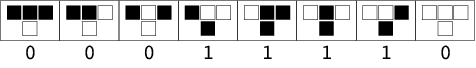
\includegraphics[scale=0.7]{resources/ElementaryCA30Rules_750.png}
			\caption{Comportamiento de la regla 30}\label{fig:picture}
		\end{figure}
		En la imagen 3 podemos ver 8 figuras diferentes entre si, si vemos la primera fila compuesta de 3 células son las combinaciones posibles de los estados (0 o 1, blanco o negro) la célula de abajo nos da el estado que poseerá la hija de la siguiente iteración, es decir, si encontramos 3 células con estado 1 (color negro) en la siguiente iteración nos generaran una célula con el estado 0 (color blanco) o por ejemplo si encontramos que nuestras dos primeras células tienen estado 0 y la ultima tiene el estado 1 entonces la célula de la próxima iteración tendrá el valor 1.\par

		Para el desarrollo de este programa se uso el lenguaje de programación Python usando Tkinter y Matplotlib para la creación de nuestra GUI y las gráficas correspondientes, el entorno de desarrollo utilizado fue Visual Studio Code. Mencionar que aunque nuestro programa nos permite usar cualquiera de las 256 reglas, en esta ocasión solo nos enfocaremos en la regla 30. Mencionar que nuestro archivo principal y el que se debe de ejecutar es el archivo con el nombre Interfaz.py ya que el archivo Logica.py solo contiene la parte lógica del programa y parte de la graficacón de los resultados.
		\newpage
		\subsection{Pruebas}
		Este programa tiene varios aspectos que han sido cubiertos. Para iniciar las pruebas
crearemos un autómata de 1000 células con 1000 iteraciones, algo especial de este autómata es que tenemos solo una célula con valor 1 en medio de todas las demás células que tienen valor 0.
		\begin{figure}[H]
			\centering
			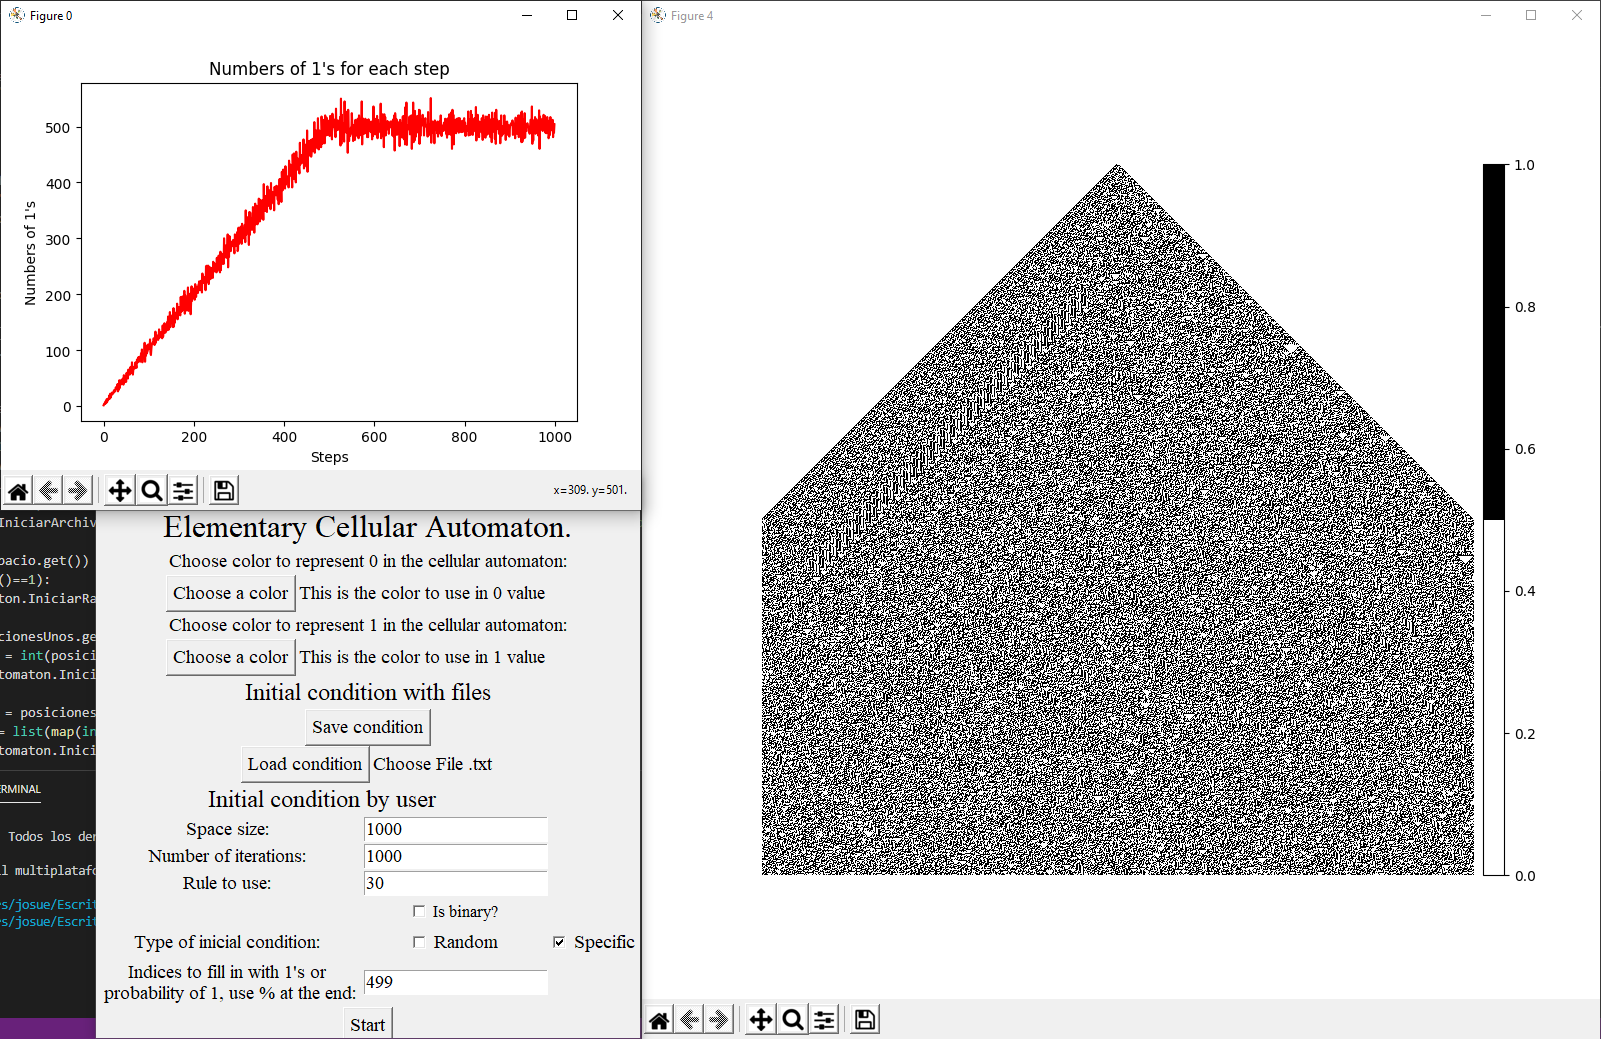
\includegraphics[scale=0.42]{resources/prueba1.png}
			\caption{ECA con solo una célula con valor 1. Regla 30}\label{fig:picture}
		\end{figure}
		Como vemos en la figura 4 tenemos en el lado derecho de la imagen nuestro ECA resultante después de aplicar 1000 iteraciones con la regla 30 y en la parte superior izquierda tenemos el crecimiento de células con valor 1 durante esas 1000 iteraciones, podemos apreciar que su crecimiento nos recuerda a un crecimiento logarítmico. En ambas gráficas tenemos la posibilidad de agrandar el tamaño mediante el icono de la lupa que tenemos en la parte inferior de ambas ventanas, una vez seleccionada la lupa podremos seleccionar un área rectangular en nuestra gráfica para poder agrandar lo que abarque dicha área, esto con el fin de visualizar aun mejor nuestro autómata y el crecimiento de nuestras células con valor 1 como se ve en la figura 5.
		\begin{figure}[H]
			\centering
			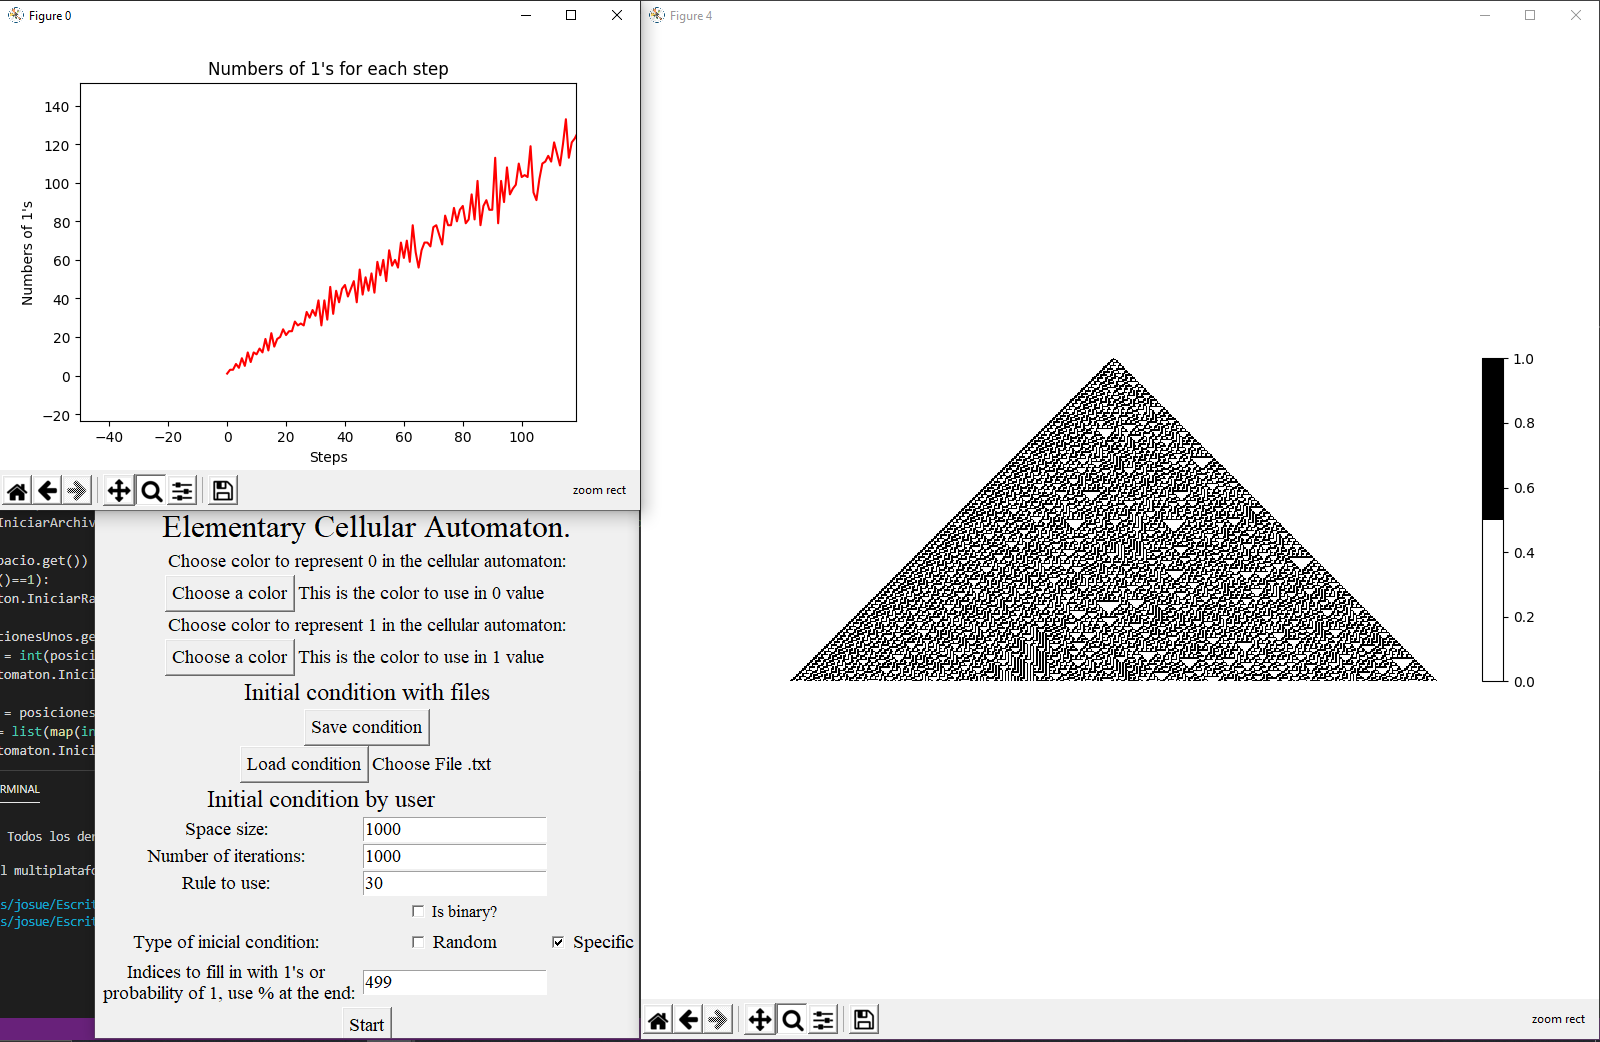
\includegraphics[scale=0.42]{resources/prueba2.png}
			\caption{ECA con solo una célula con valor 1 agrandando el tamaño para poder visualizar aun mejor el comportamiento. Regla 30}\label{fig:picture}
		\end{figure}
		Nuestro programa también nos permite guardar nuestra configuración de nuestro ECA, en este caso solo toma la iteración 0 y es guardado en un archivo con el siguiente nombre $"$celulasIniciales.txt$"$ en caso de existir sobre escribirá la nueva información, en caso contrario lo creara desde cero, mencionar que si se desea se puede modificar el nombre pero no la extensión posterior de haber creado el archivo. En este caso nuestro programa nos arroja un mensaje diciendo que el archivo fue guardo exitosamente y se nos crea un archivo con el nombre y extensión anteriormente mencionados (ver figura 6 y 7).
		\begin{figure}[H]
			\centering
			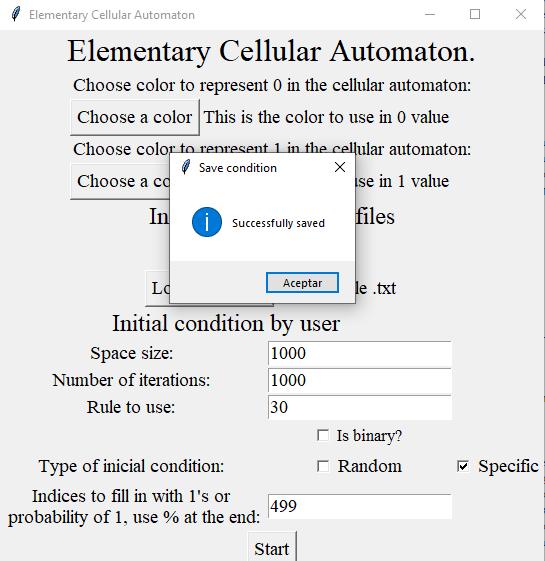
\includegraphics[scale=0.42]{resources/archivoSave.png}
			\caption{Iteración 0 de nuestro ECA guardada exitosamente}\label{fig:picture}
		\end{figure}
		\begin{figure}[H]
			\centering
			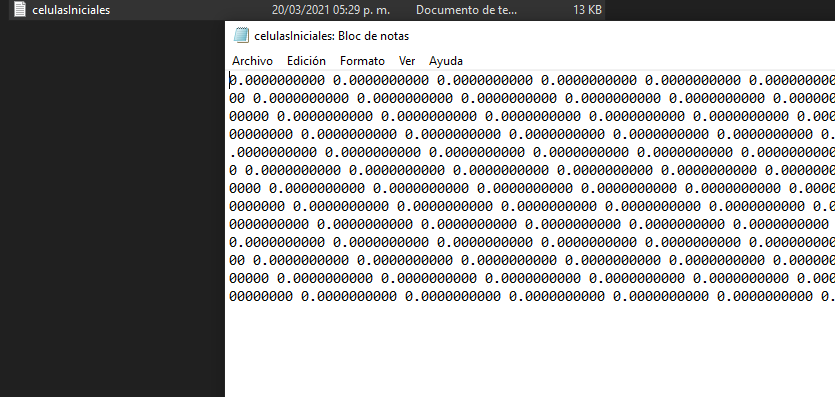
\includegraphics[scale=0.5]{resources/archivoSave2.png}
			\caption{Contenido del archivo}\label{fig:picture}
		\end{figure}
		También como era de esperarse se puede cargar archivo de texto al programa para volver a usarlo, algo importante a mencionar es que no guarda ni el numero de iteraciones, los colores para los valores 0 y 1 ni la regla usada esto con fines de facilitar al usuario poder usar un mismo inicio con diferentes reglas y numero de iteraciones cada vez que le plazca hacerlo. En la figura 8 cargamos nuestro archivo y solo modificamos el color que se le asigna a los valores 0 y 1, colocamos la regla a usar (regla 30) y nuestro numero de iteraciones sera de nuevo 1000, el panel para poder elegir el color se puede observar en la figura 9.
		\begin{figure}[H]
			\centering
			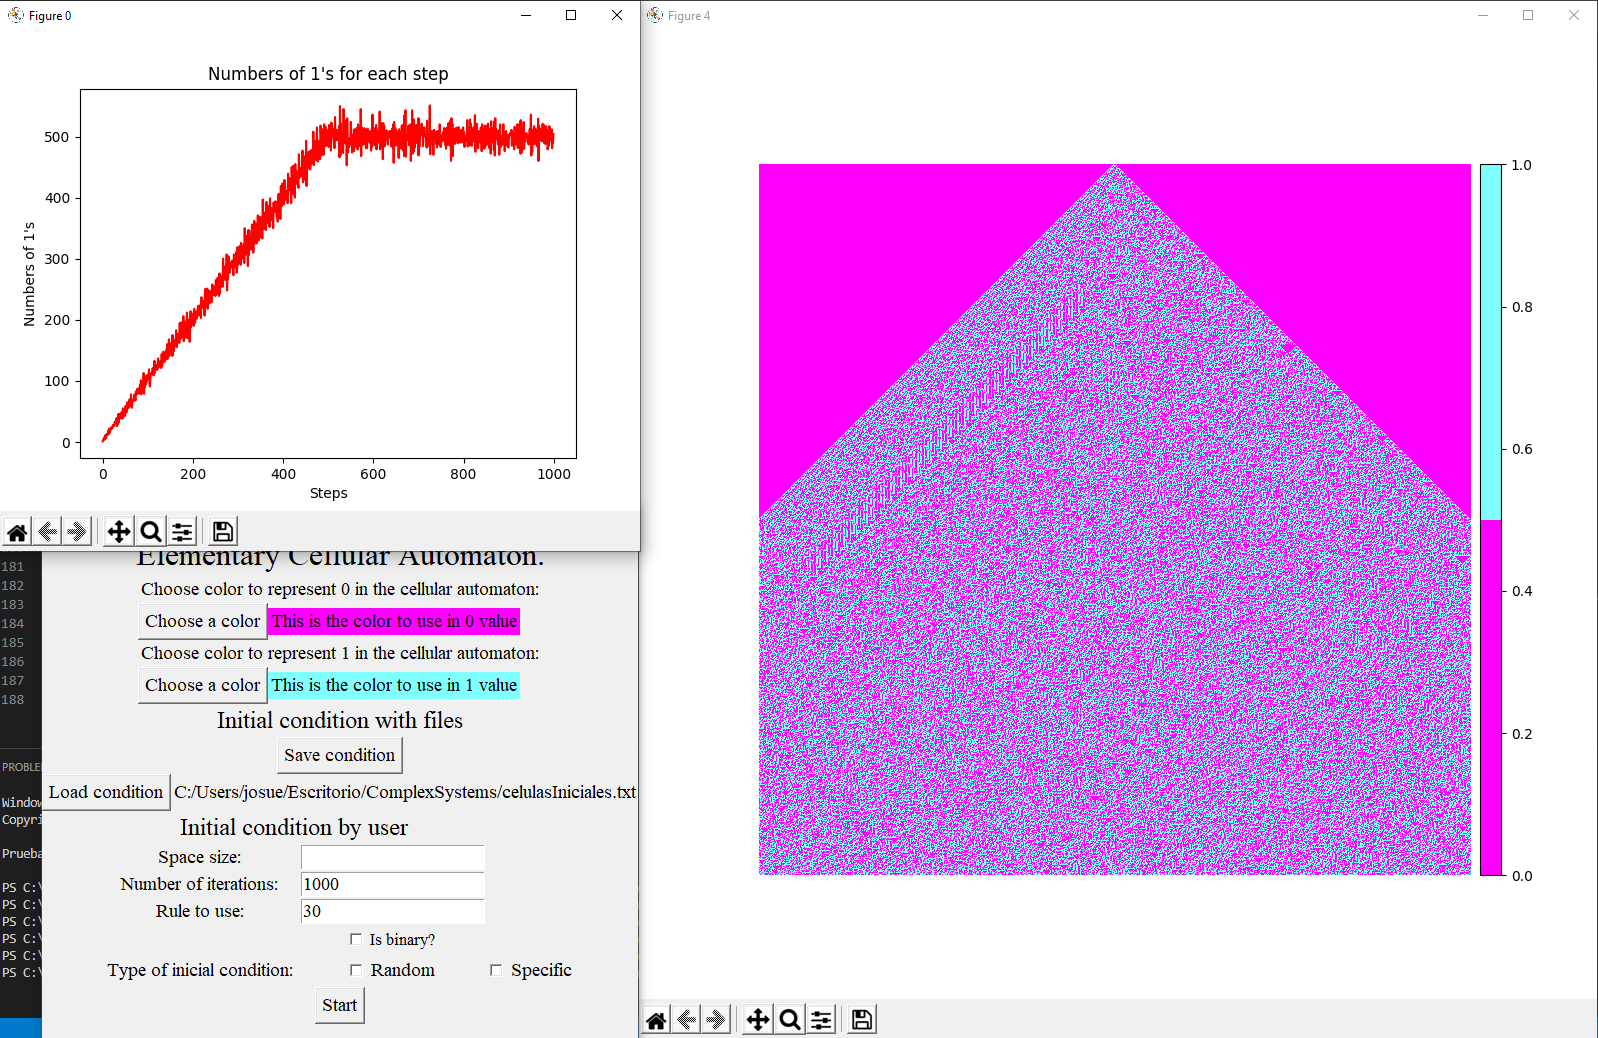
\includegraphics[scale=0.42]{resources/automataHappy.png}
			\caption{ECA con diferentes colores para los valores 0 y 1}\label{fig:picture}
		\end{figure}
		\begin{figure}[H]
			\centering
			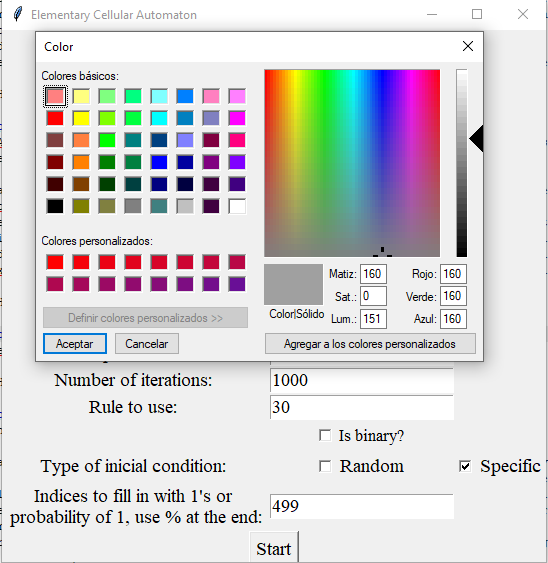
\includegraphics[scale=0.5]{resources/elegirColor.png}
			\caption{Panel para poder elegir color para valores 0 y 1}\label{fig:picture}
		\end{figure}
		Realizando otra prueba crearemos un ECA con un tamaño de 500 células con 500 iteraciones, pero en esta ocasión la regla 30 sera ingresada como numero binario (00011110$_2$) y serán asignadas células con valor 1 de forma aleatoria.
		\begin{figure}[H]
			\centering
			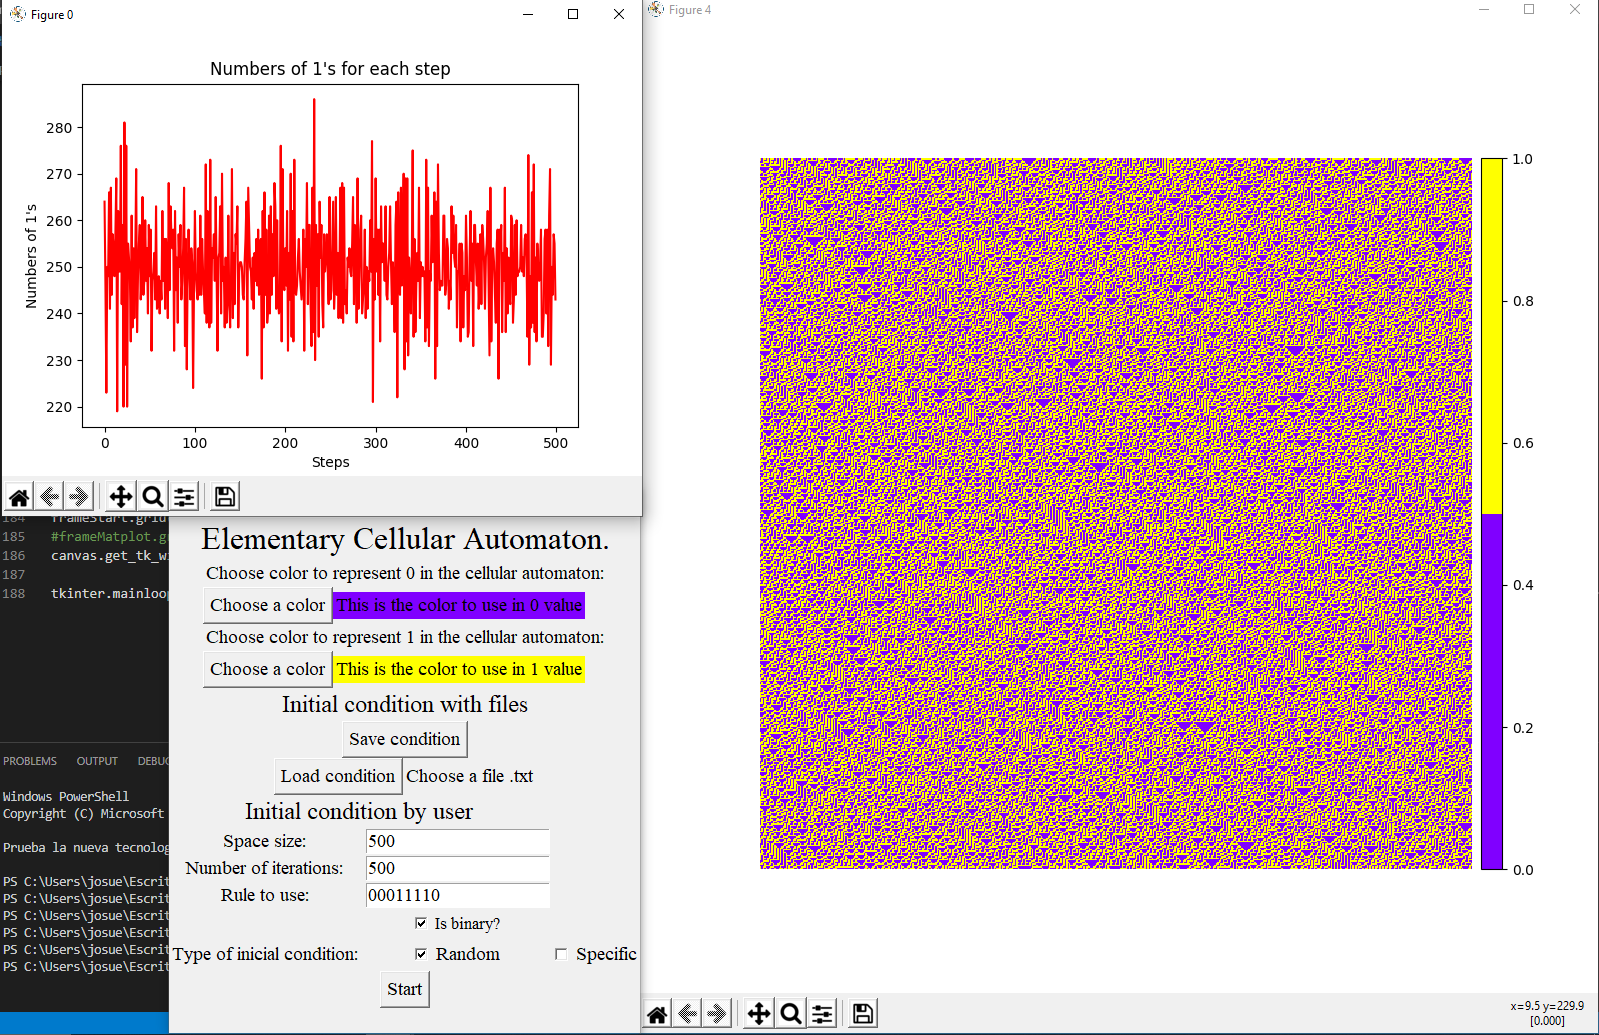
\includegraphics[scale=0.42]{resources/pruebaF.png}
			\caption{ECA de 500 células por 500 iteraciones creado de forma aleatoria}								\label{fig:picture}
		\end{figure}
		Como ultimas pruebas realizaremos lo siguiente:  mediante las reglas 15, 22, 30, 54, 110 y 126 para la construcción de nuestro ECA mostraremos 3 evoluciones por cada regla en espacios de 400 células por 400 iteraciones, una empezara con un uno al centro, otra iniciando con un 50\% de probabilidad de unos y la última iniciando con un 95\% de probabilidad de unos.\par
		Empecemos así con nuestra regla 15, veremos a través de de las imágenes 11 a la 14 el comportamiento de nuestro ECA con base en donde se encuentren las células iniciales con valor 1.
		\begin{figure}[H]
			\centering
			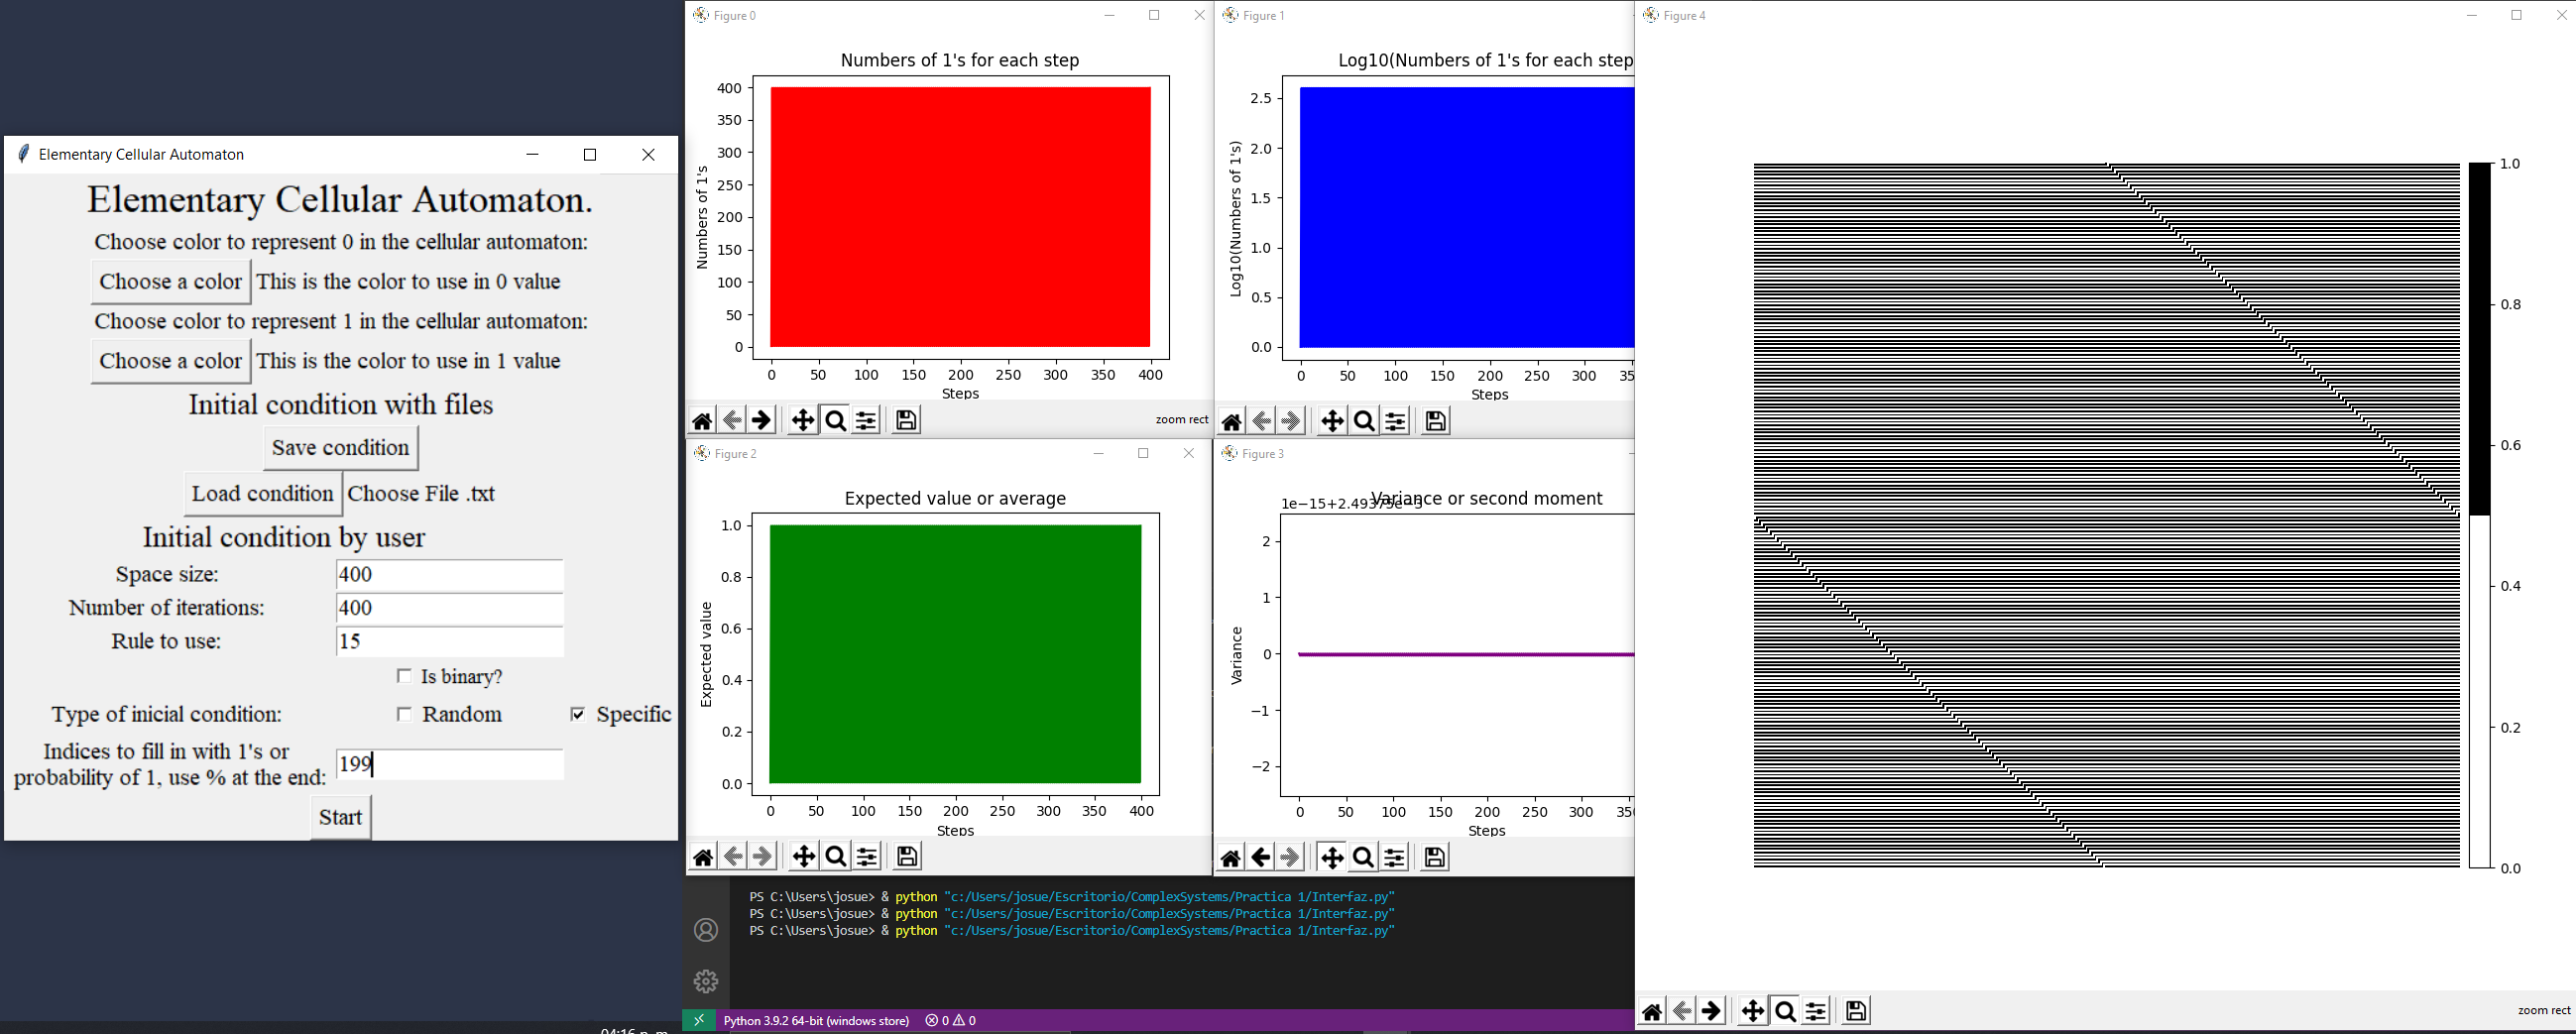
\includegraphics[scale=0.26]{resources/add1.png}
			\caption{ECA de 400 células por 400 iteraciones con una célula inicial central, regla 15}								\label{fig:picture}
		\end{figure}
		Para visualizar mejor la información nuestras gráficas hagamos una ampliación de las mismas para las primeras 50 iteraciones.
		\begin{figure}[H]
			\centering
			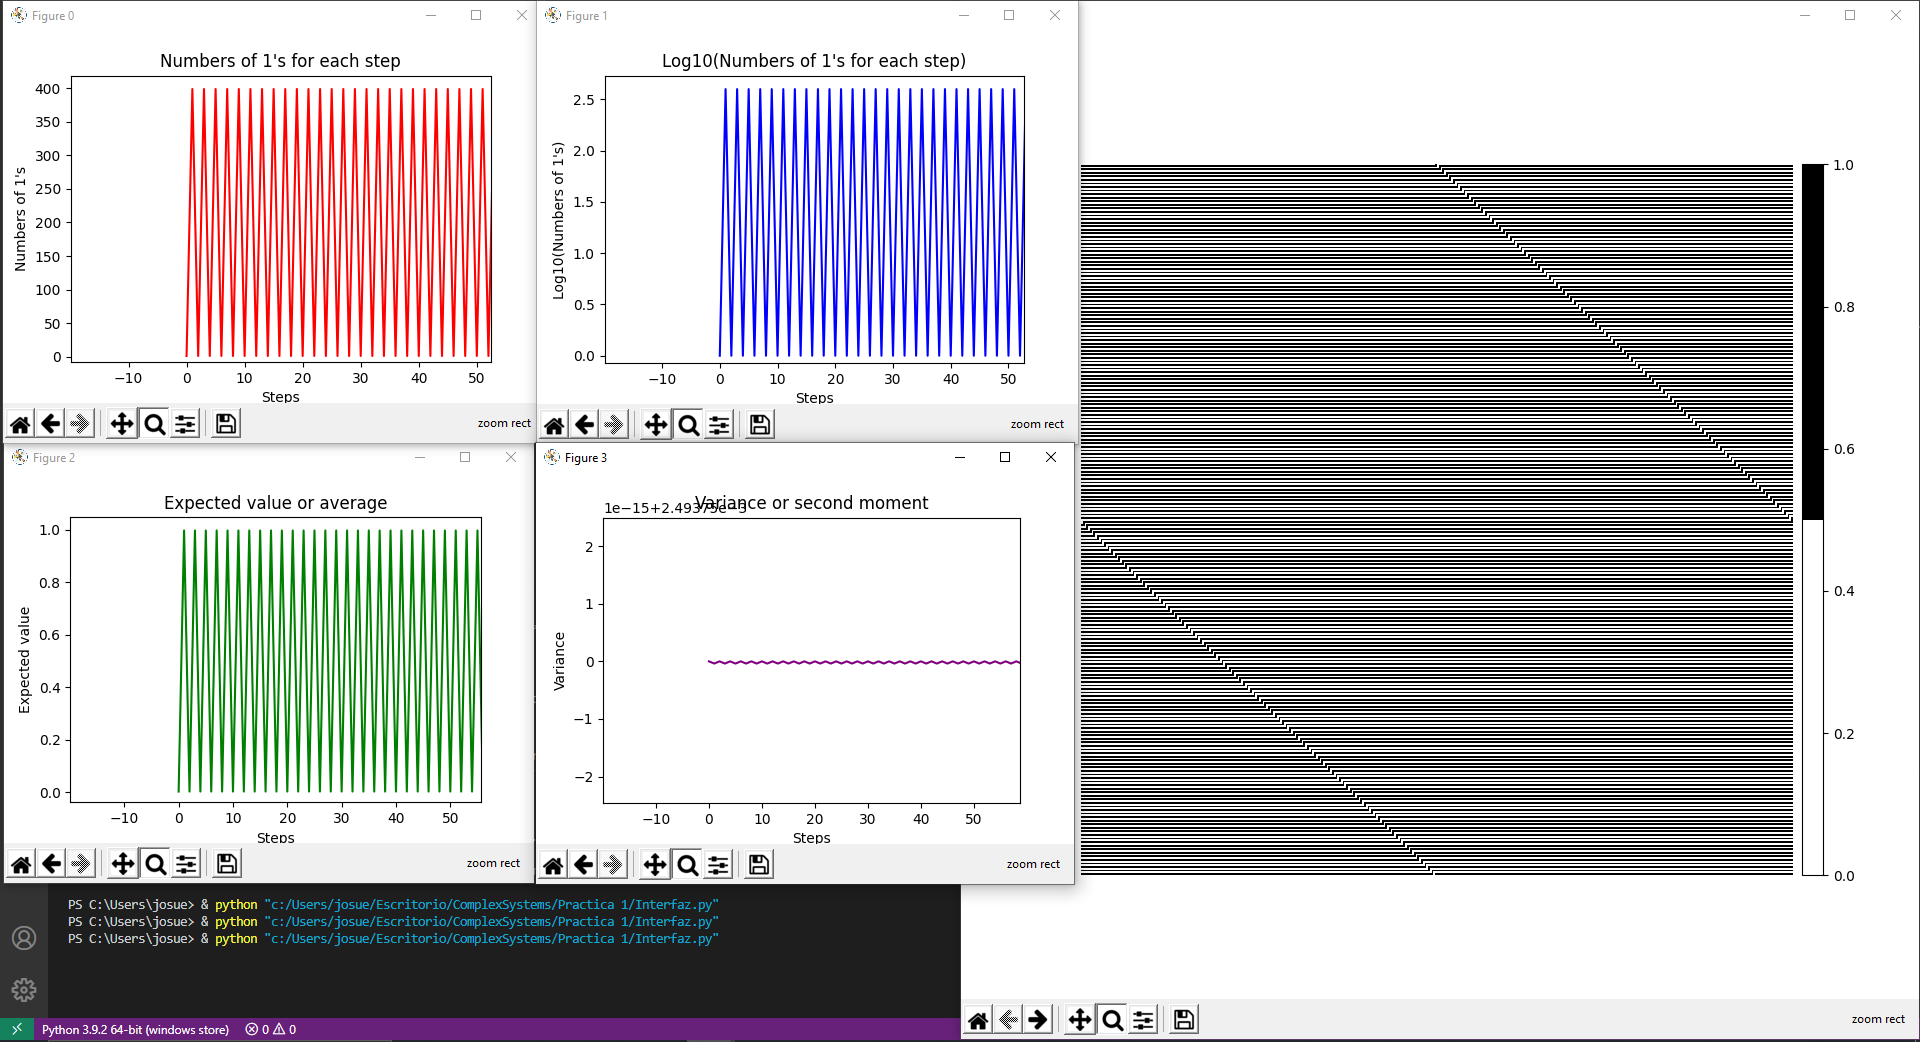
\includegraphics[scale=0.35]{resources/add1z.png}
			\caption{ECA de 400 células por 400 iteraciones con una célula inicial central con aumento, regla 15}								\label{fig:picture}
		\end{figure}
		Como vemos el comportamiento de nuestro ECA es de una forma constante y es que en la iteración tenemos 1 célula viva a pasar a tener 399 células y a la siguiente volvemos a tener solo una, como si de un ciclo se tratase.\par
		Pasando a la siguiente prueba, usaremos el 50\% de unos y observemos su comportamiento
		\begin{figure}[H]
			\centering
			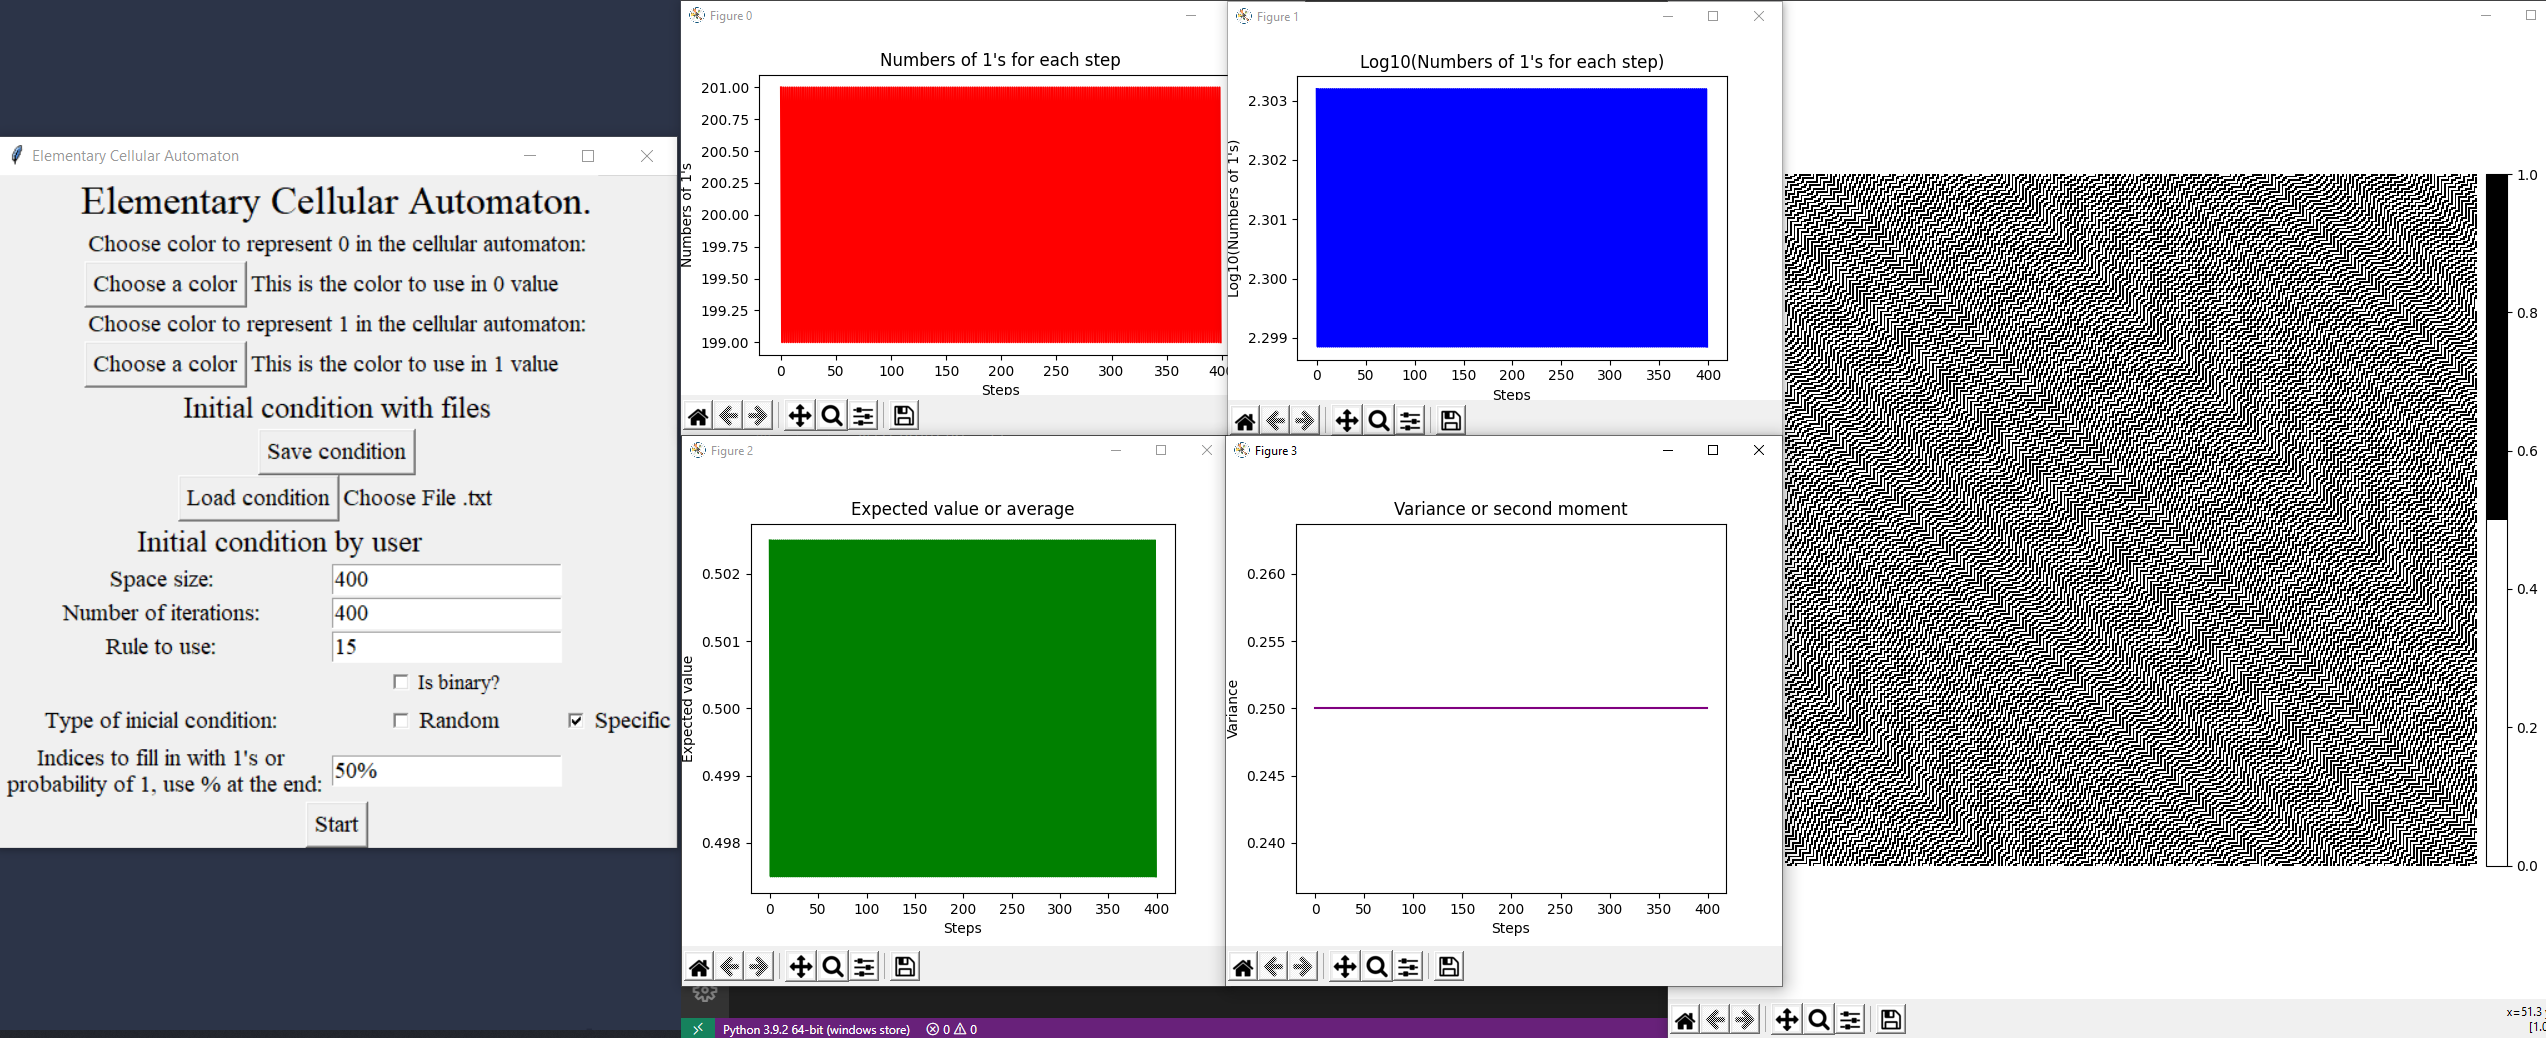
\includegraphics[scale=0.26]{resources/add2.png}
			\caption{ECA de 400 células por 400 iteraciones con 50\% de probabilidad de 1's, regla 15}								\label{fig:picture}
		\end{figure}		
		Como vemos tiene un comportamiento similar a la primera prueba solo que el numero de células vivas por iteración cambiaron, ahora son menos que en la prueba anterior.
		Como ultima prueba para esta regla, la probabilidad a usar sera del 95\% así que veamos el resultado
		\begin{figure}[H]
			\centering
			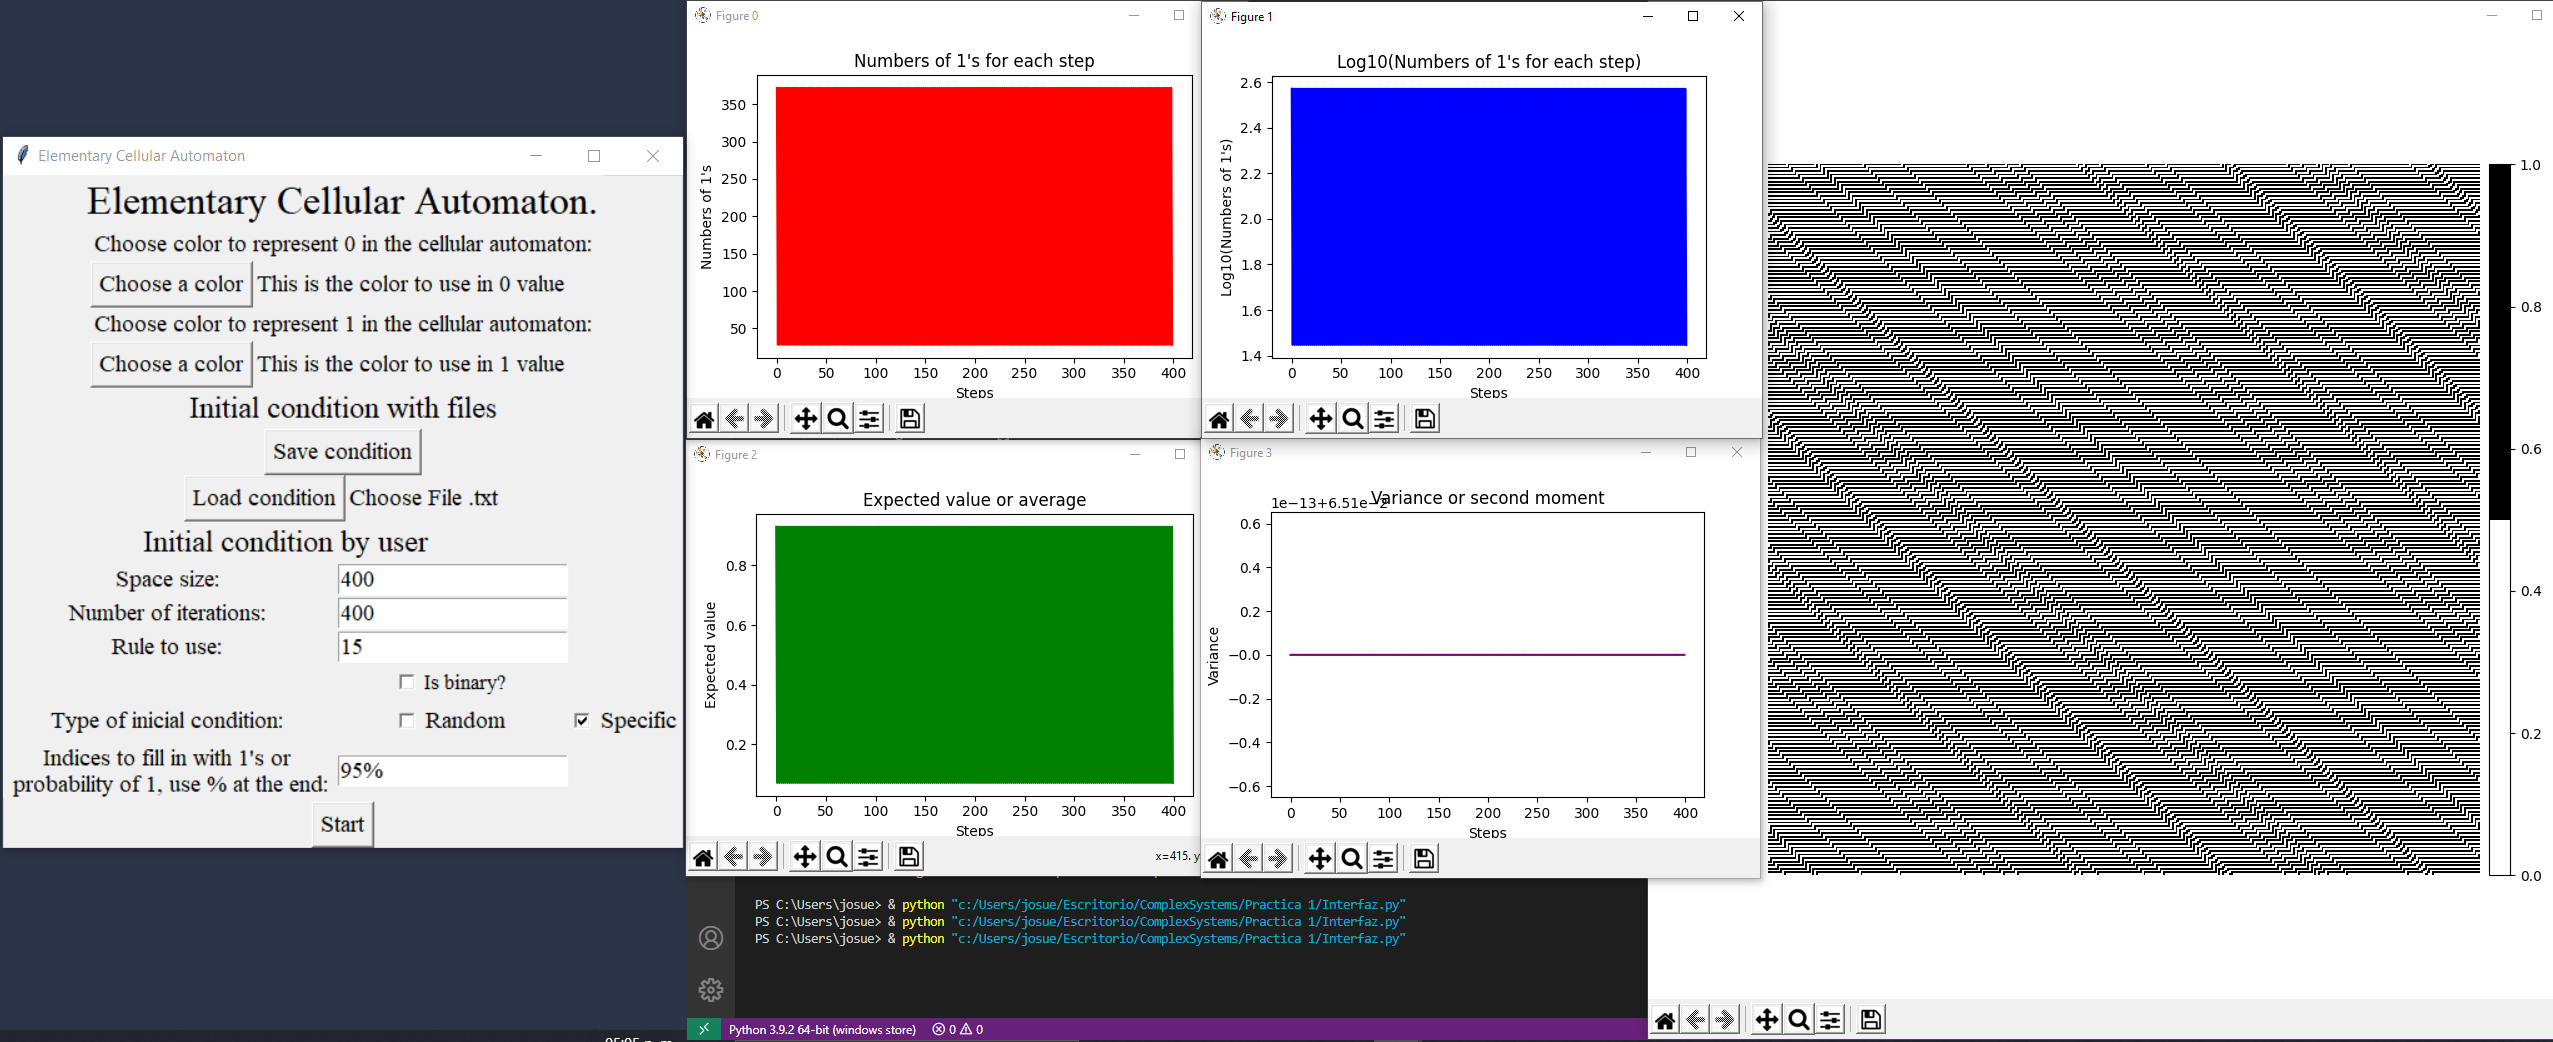
\includegraphics[scale=0.26]{resources/add3.png}
			\caption{ECA de 400 células por 400 iteraciones con 95\% de probabilidad de 1's, regla 15}								\label{fig:picture}
		\end{figure}		
		El resultado nuevamente es muy similar a los anteriores, por lo que podemos suponer que si probamos diferentes configuraciones iniciales siempre serán parecidas, solo cambiaran el numero de 1's.\par
		Continuando con las pruebas, ahora vayamos con la regla 22 de aquí en adelante se mostraran las 3 imágenes correspondientes con los 3 valores iniciales diferentes para posteriormente dar un pequeño estudio de los resultados.
		\begin{figure}[H]
			\centering
			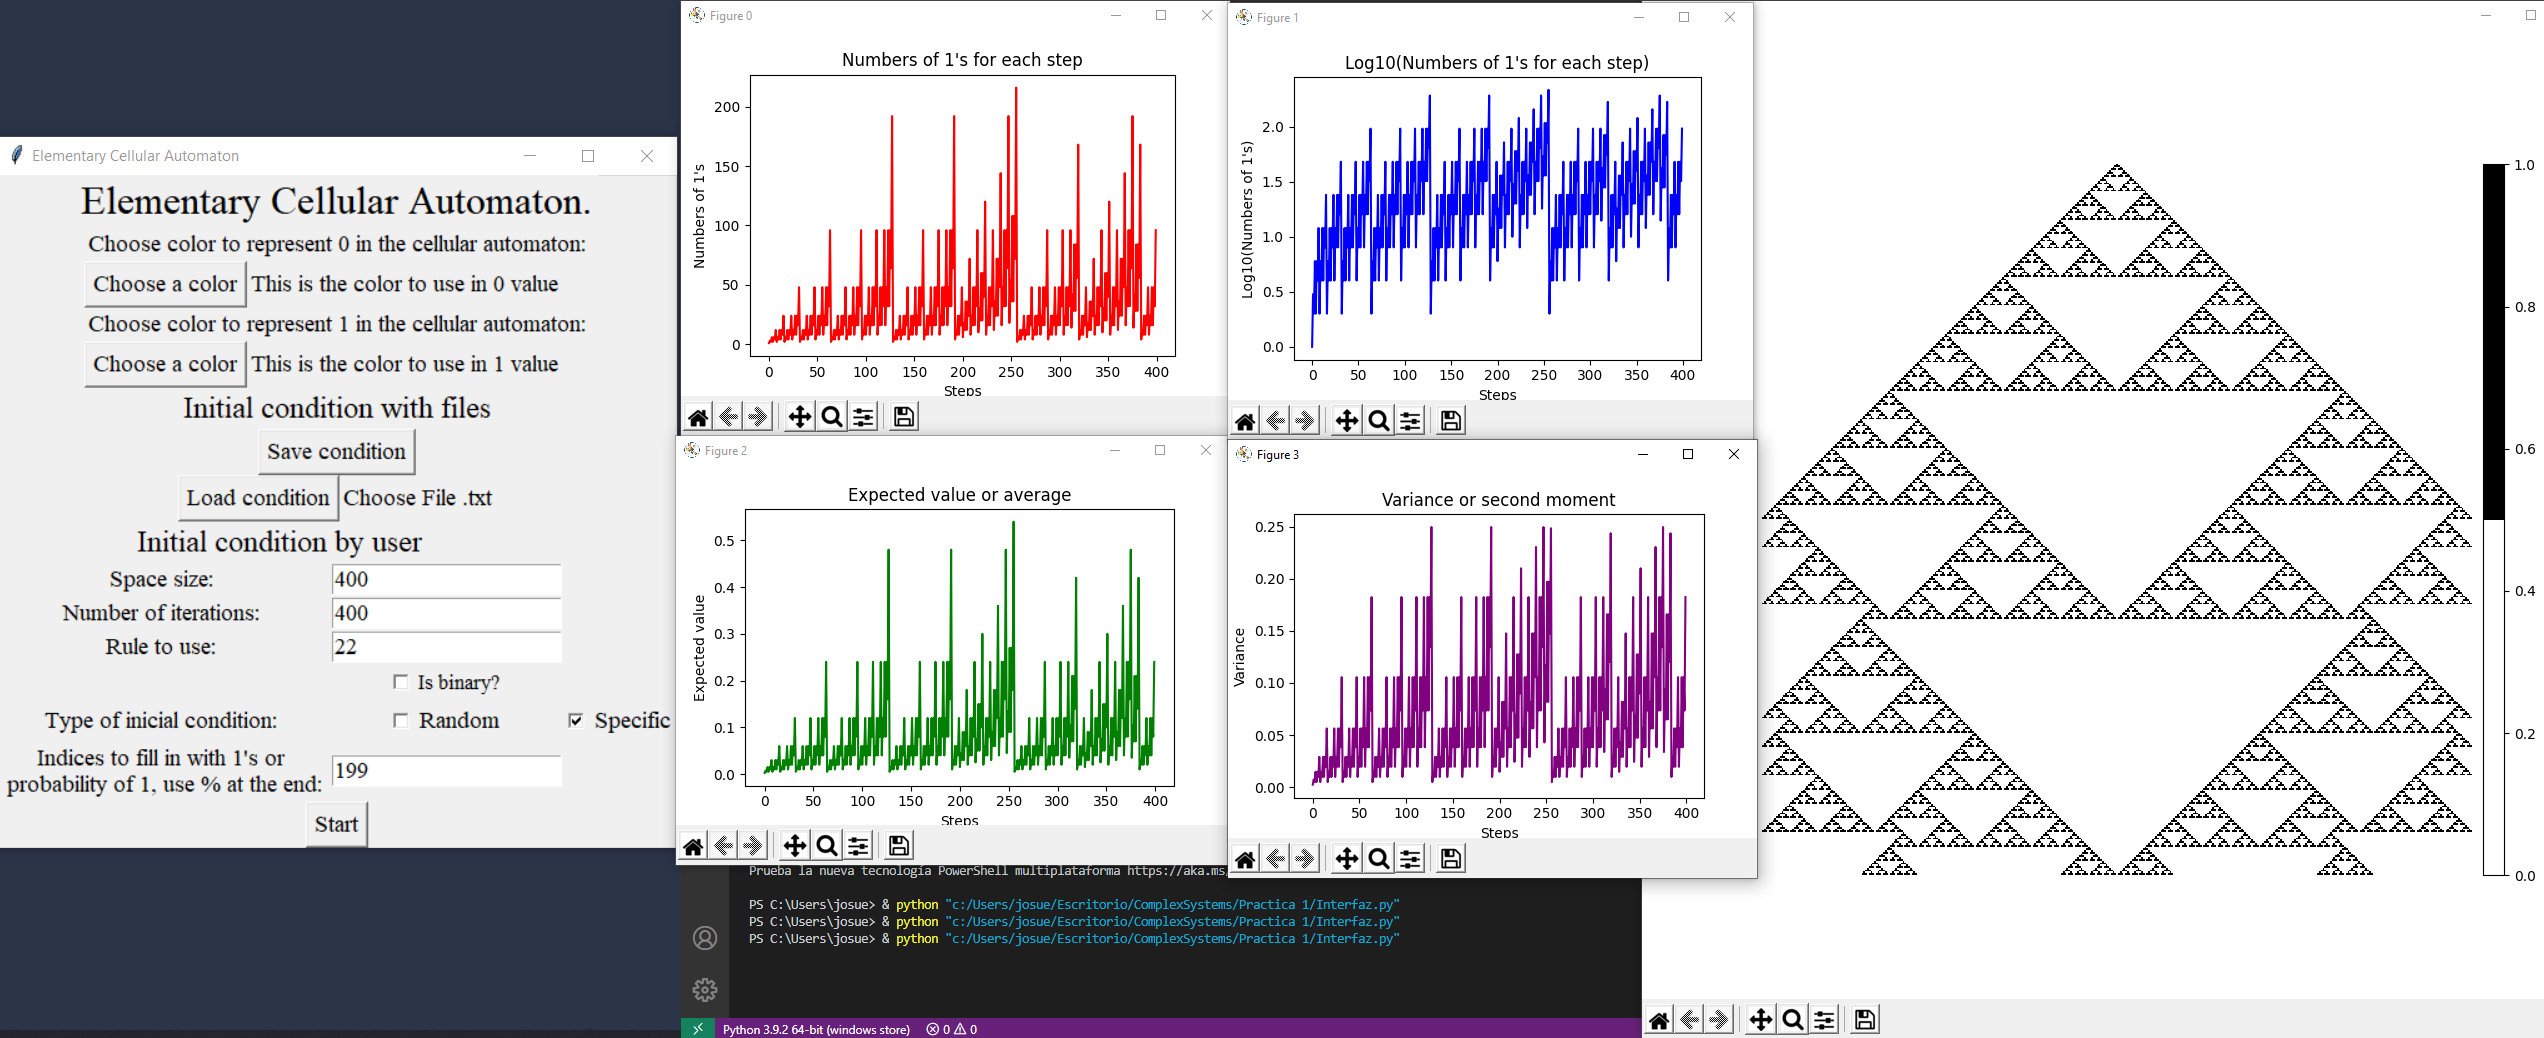
\includegraphics[scale=0.26]{resources/add4.png}
			\caption{ECA de 400 células por 400 iteraciones con una célula inicial central, regla 22}								\label{fig:picture}
		\end{figure}
		\begin{figure}[H]
			\centering
			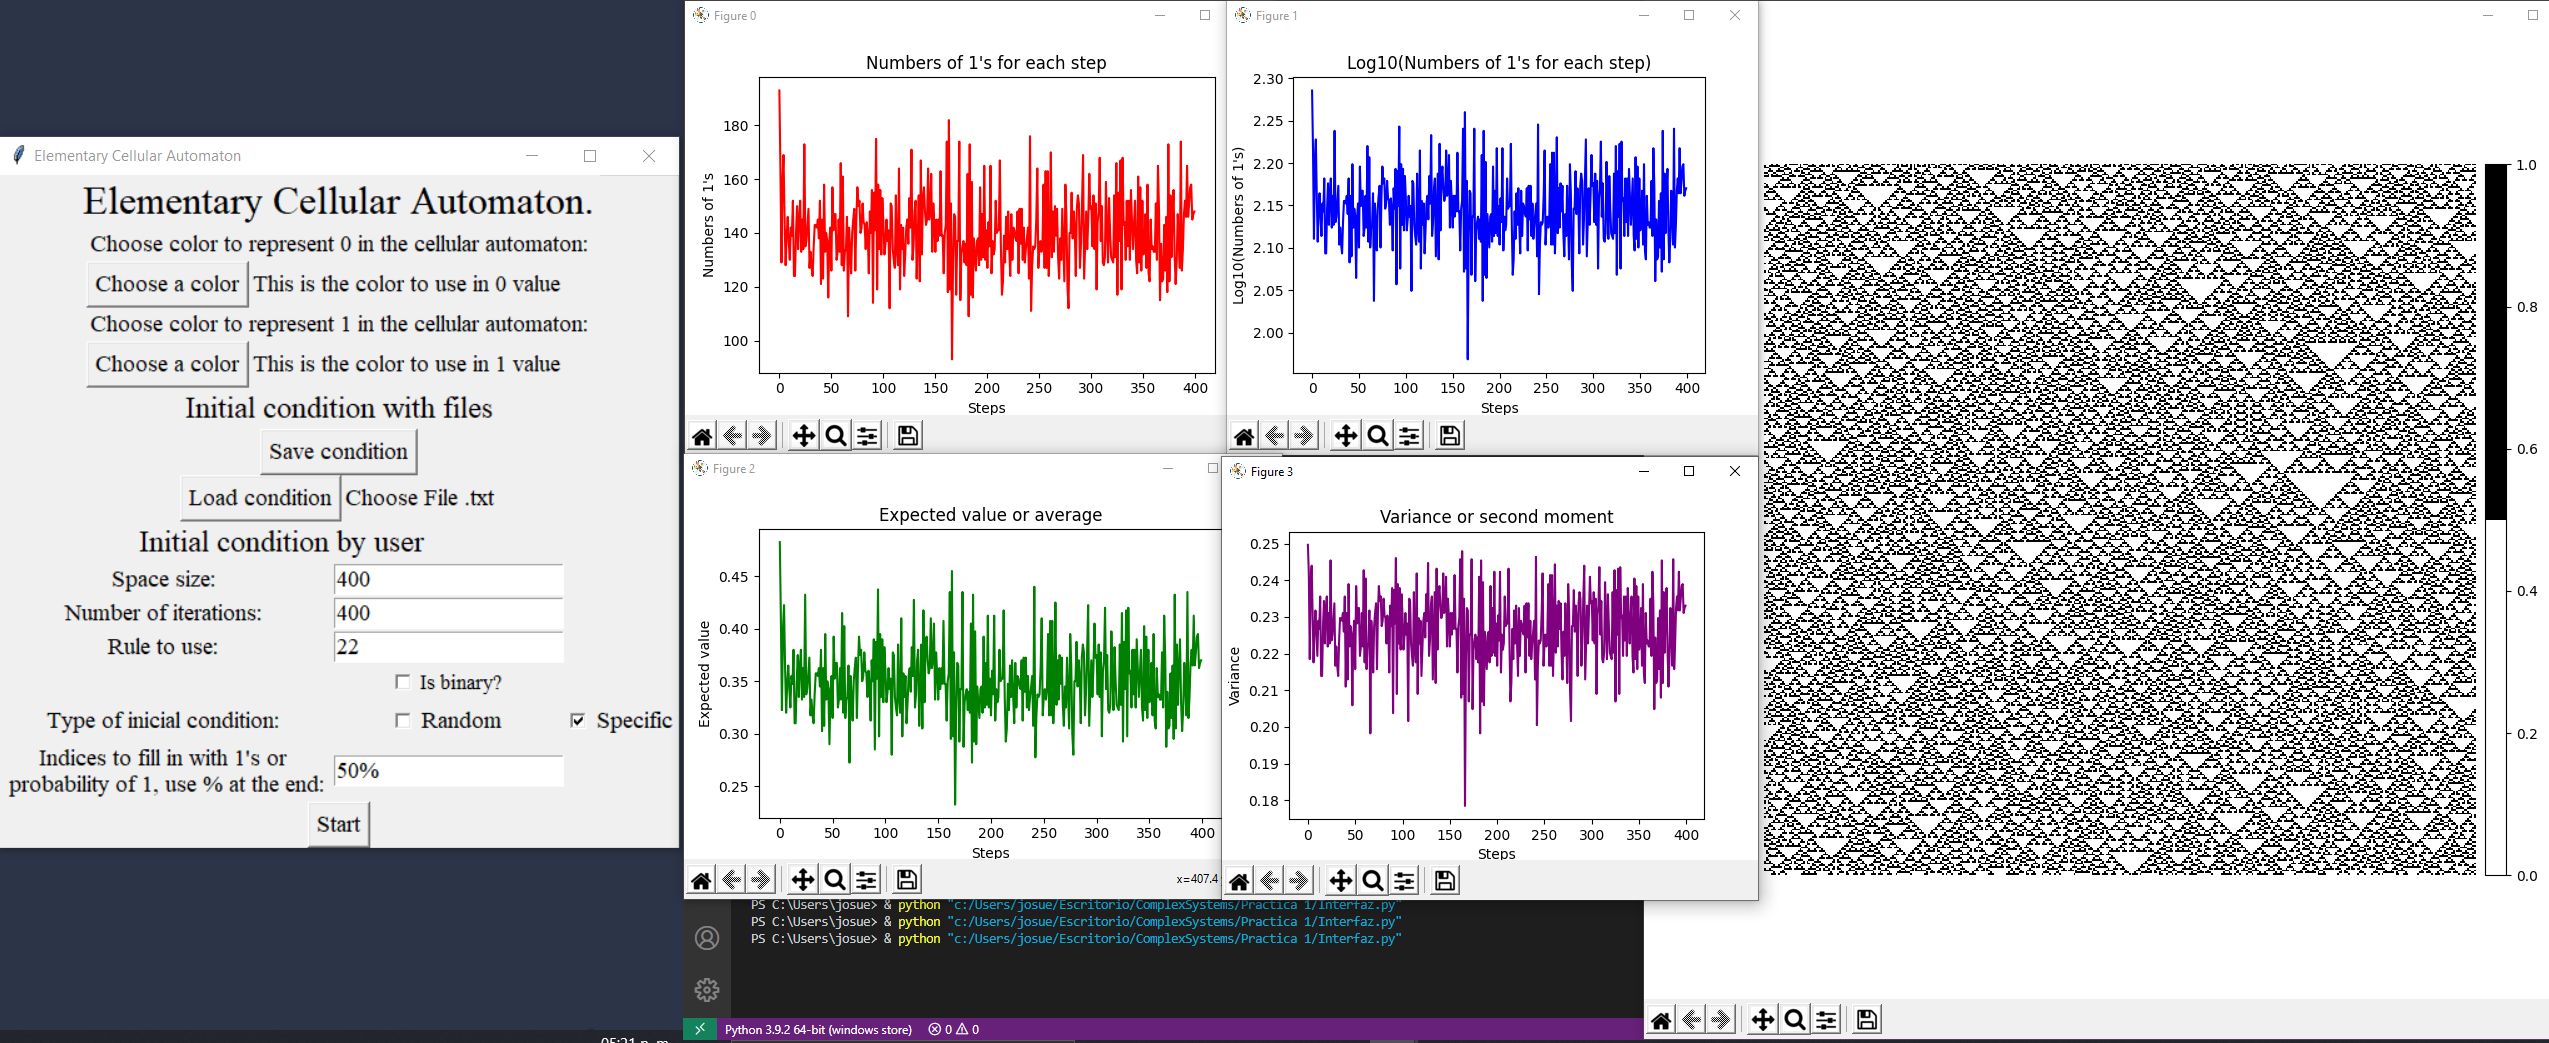
\includegraphics[scale=0.26]{resources/add5.png}
			\caption{ECA de 400 células por 400 iteraciones con 50\% de probabilidad de 1's, regla 22}								\label{fig:picture}
		\end{figure}
		\begin{figure}[H]
			\centering
			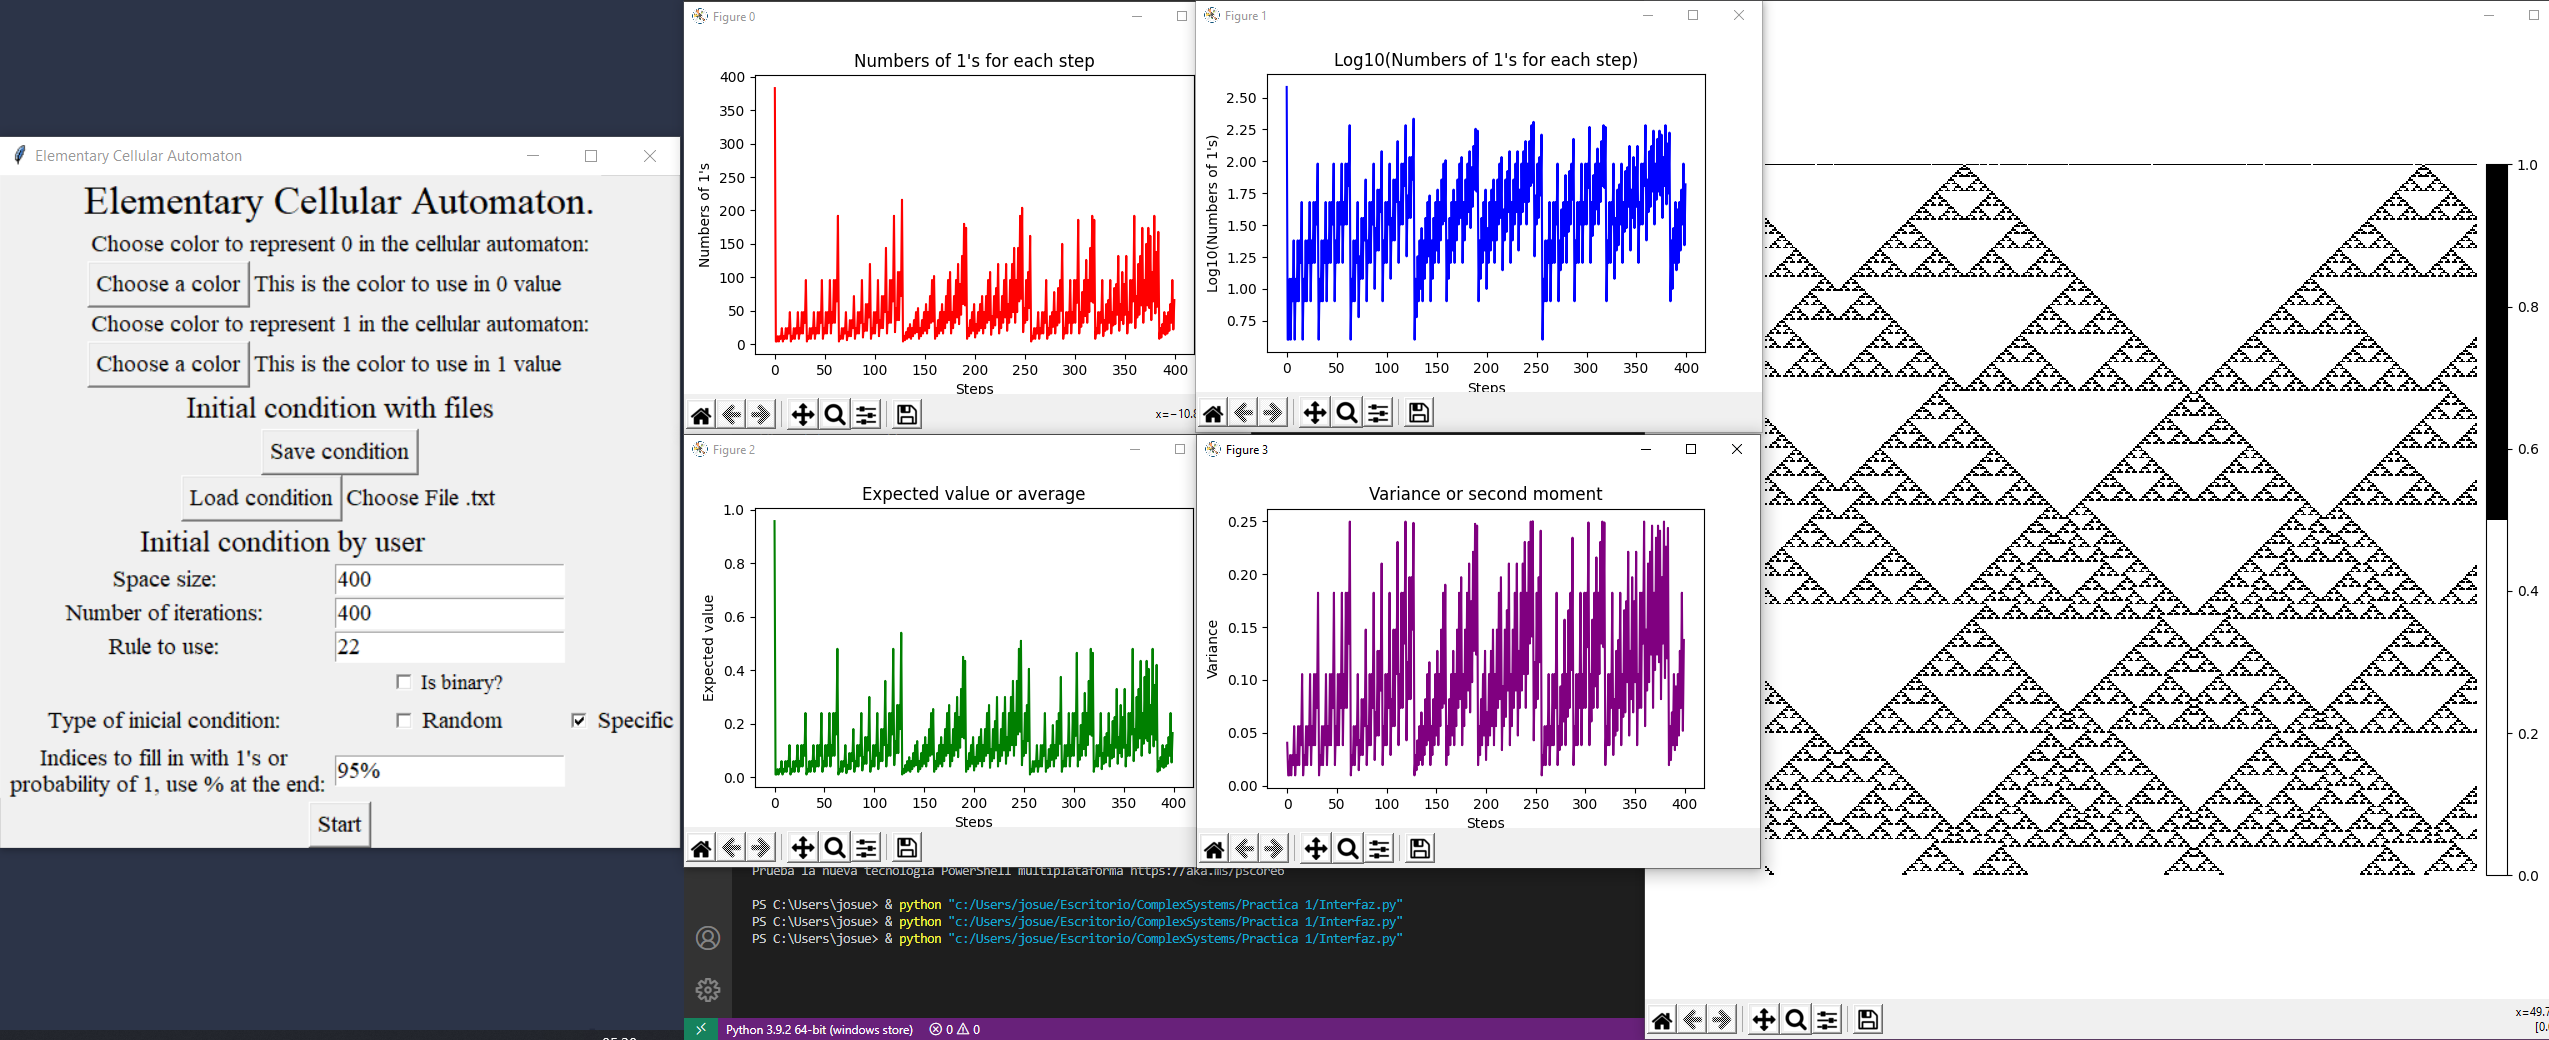
\includegraphics[scale=0.26]{resources/add6.png}
			\caption{ECA de 400 células por 400 iteraciones con 95\% de probabilidad de 1's, regla 22}								\label{fig:picture}
		\end{figure}
		Como se ven desde la figura 15 a la 17 con esta regla si cambia el comportamiento de nuestras gráficas con base a cada tipo de condición inicial, aunque la figura 15 y 17 tiene ciertas similitudes pero no son lo mismo, empezamos a ver que tan influyente es la regla en el comportamiento de nuestro ECA. \par 
		Ahora pasemos a la regla 30 con las mismas pruebas.
		\begin{figure}[H]
			\centering
			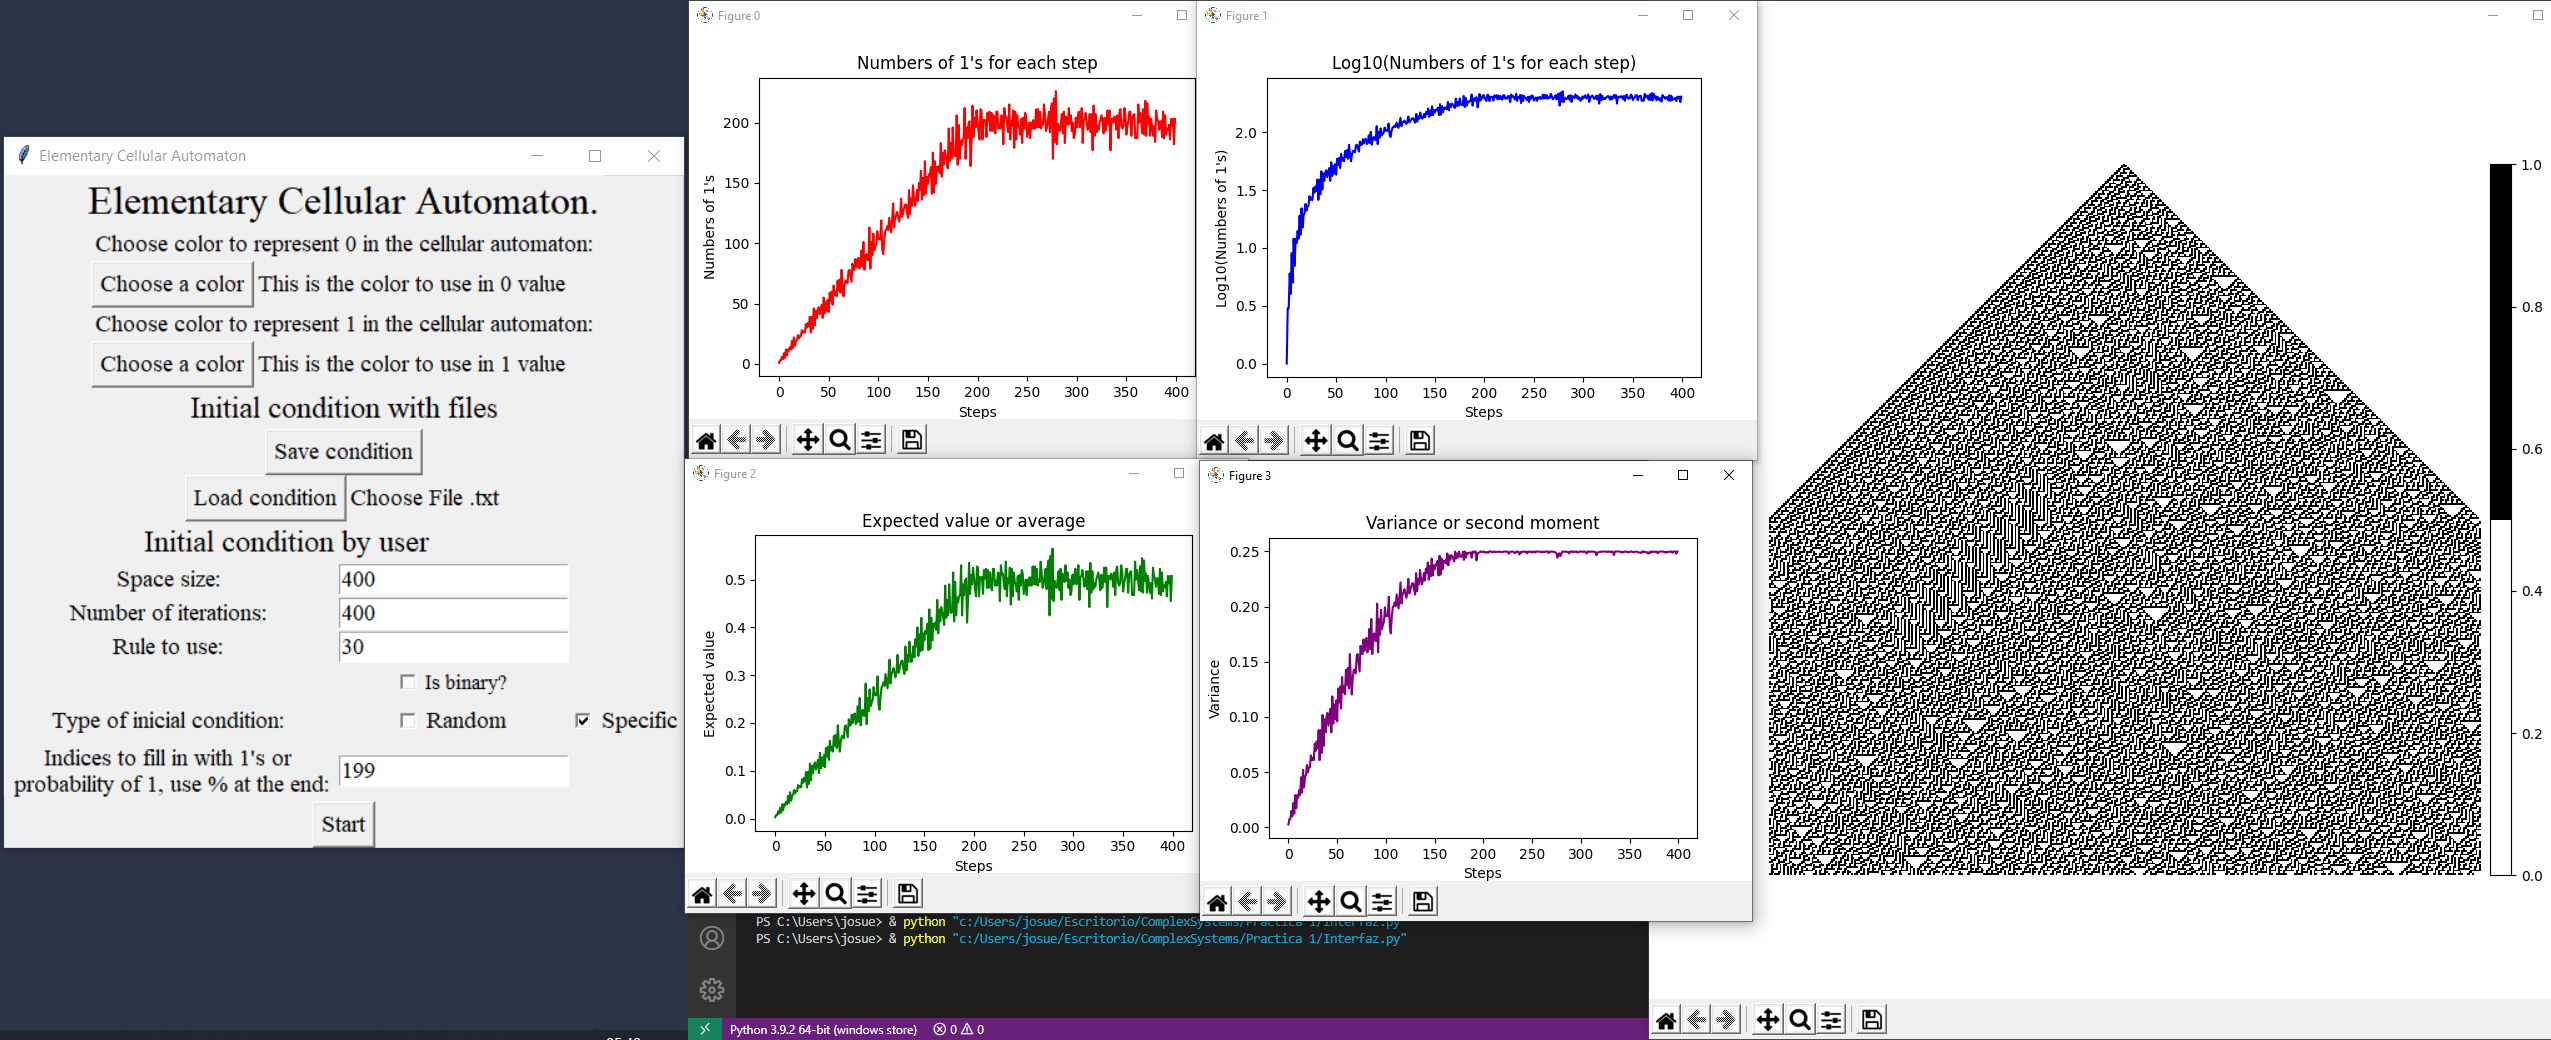
\includegraphics[scale=0.26]{resources/add7.png}
			\caption{ECA de 400 células por 400 iteraciones con una célula inicial central, regla 30}								\label{fig:picture}
		\end{figure}
		\begin{figure}[H]
			\centering
			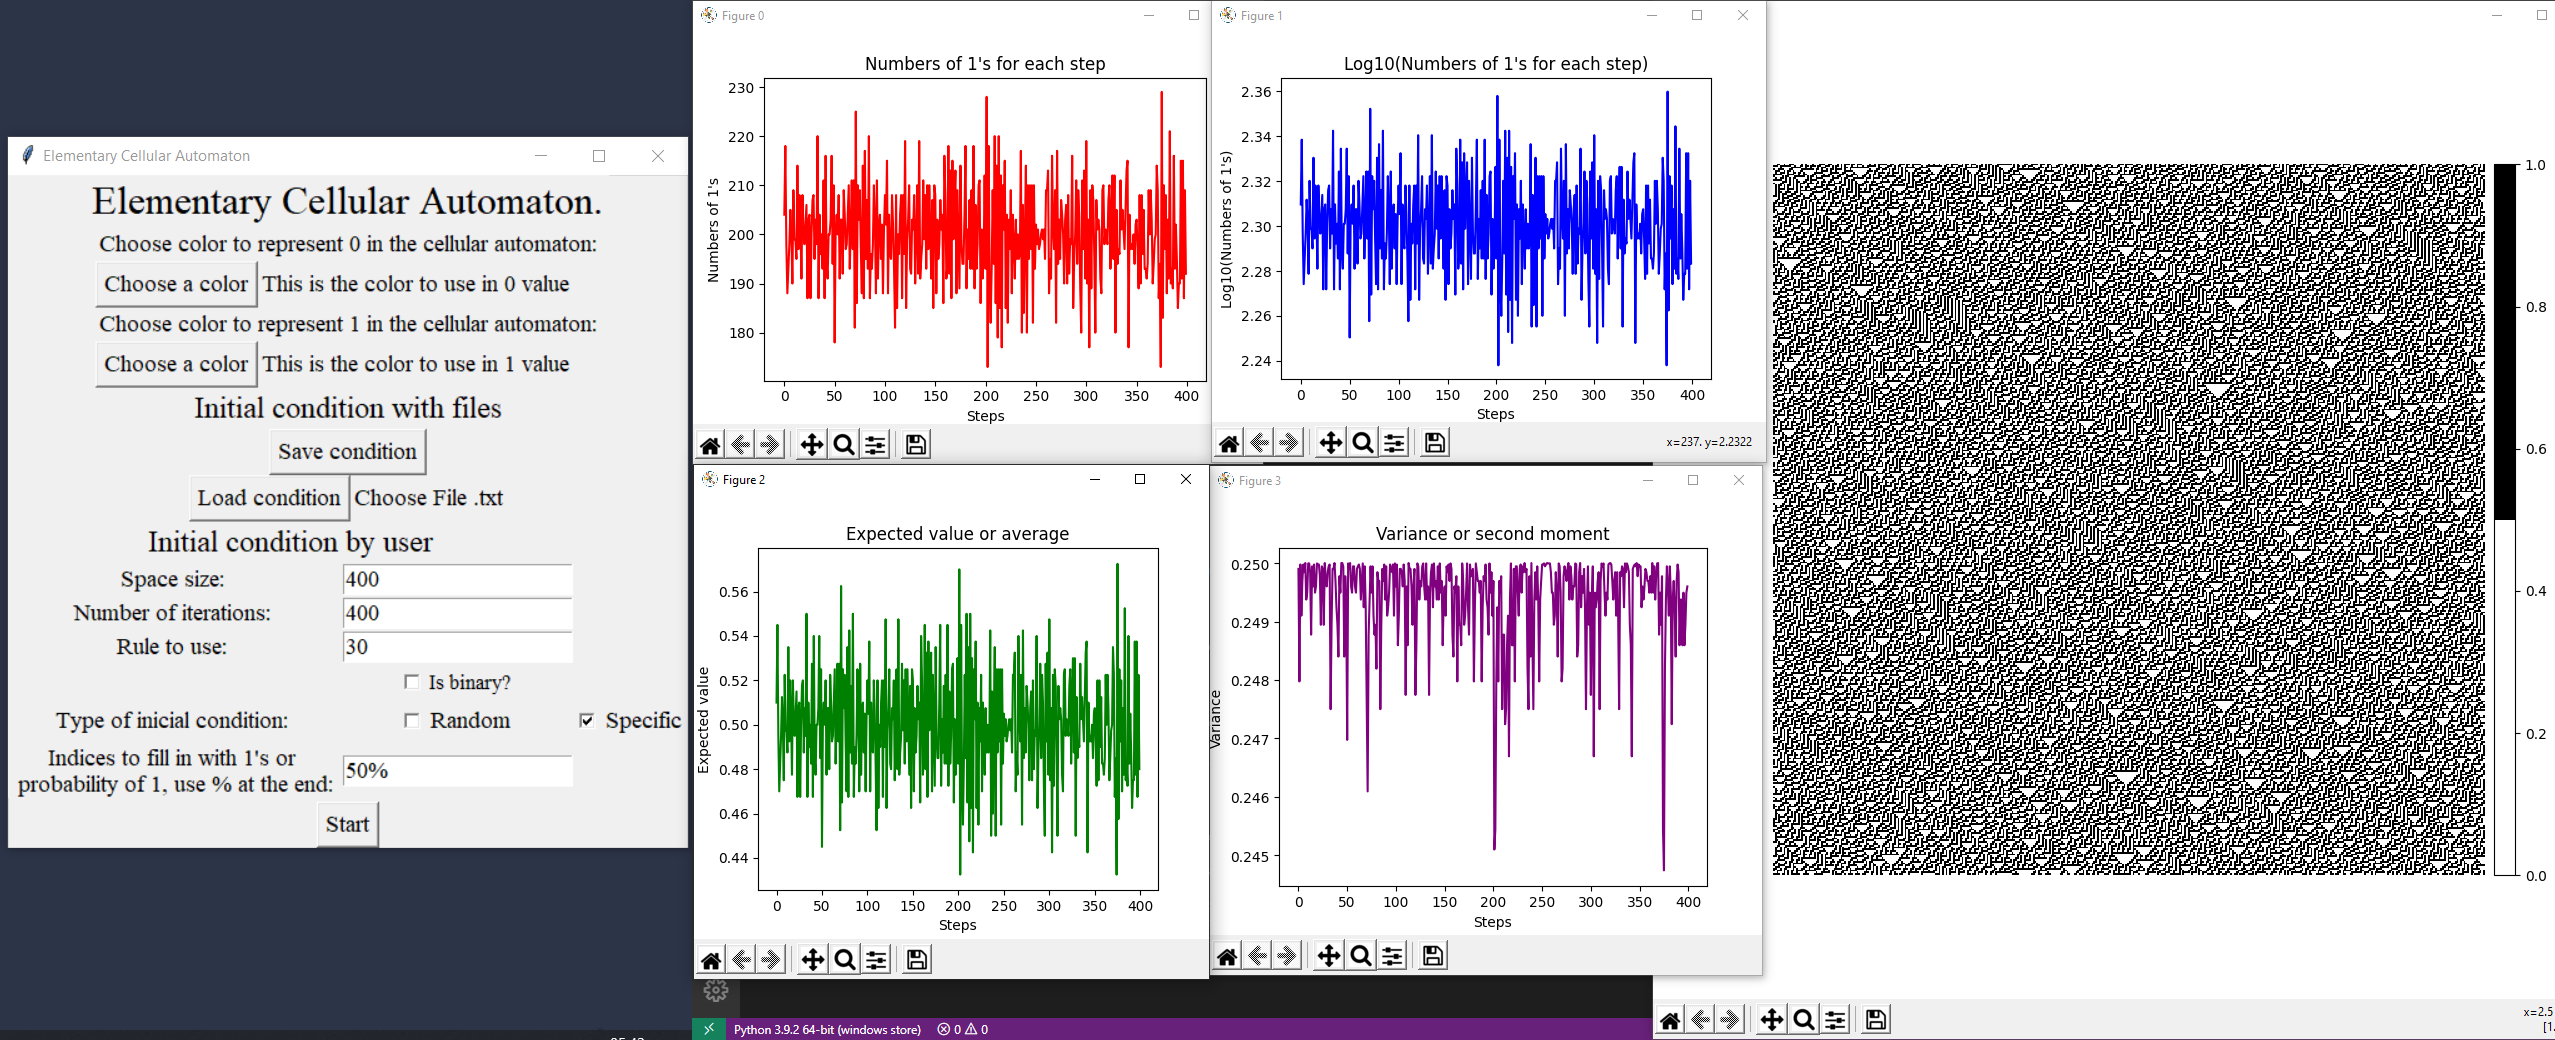
\includegraphics[scale=0.26]{resources/add8.png}
			\caption{ECA de 400 células por 400 iteraciones con 50\% de probabilidad de 1's, regla 30}								\label{fig:picture}
		\end{figure}
		\begin{figure}[H]
			\centering
			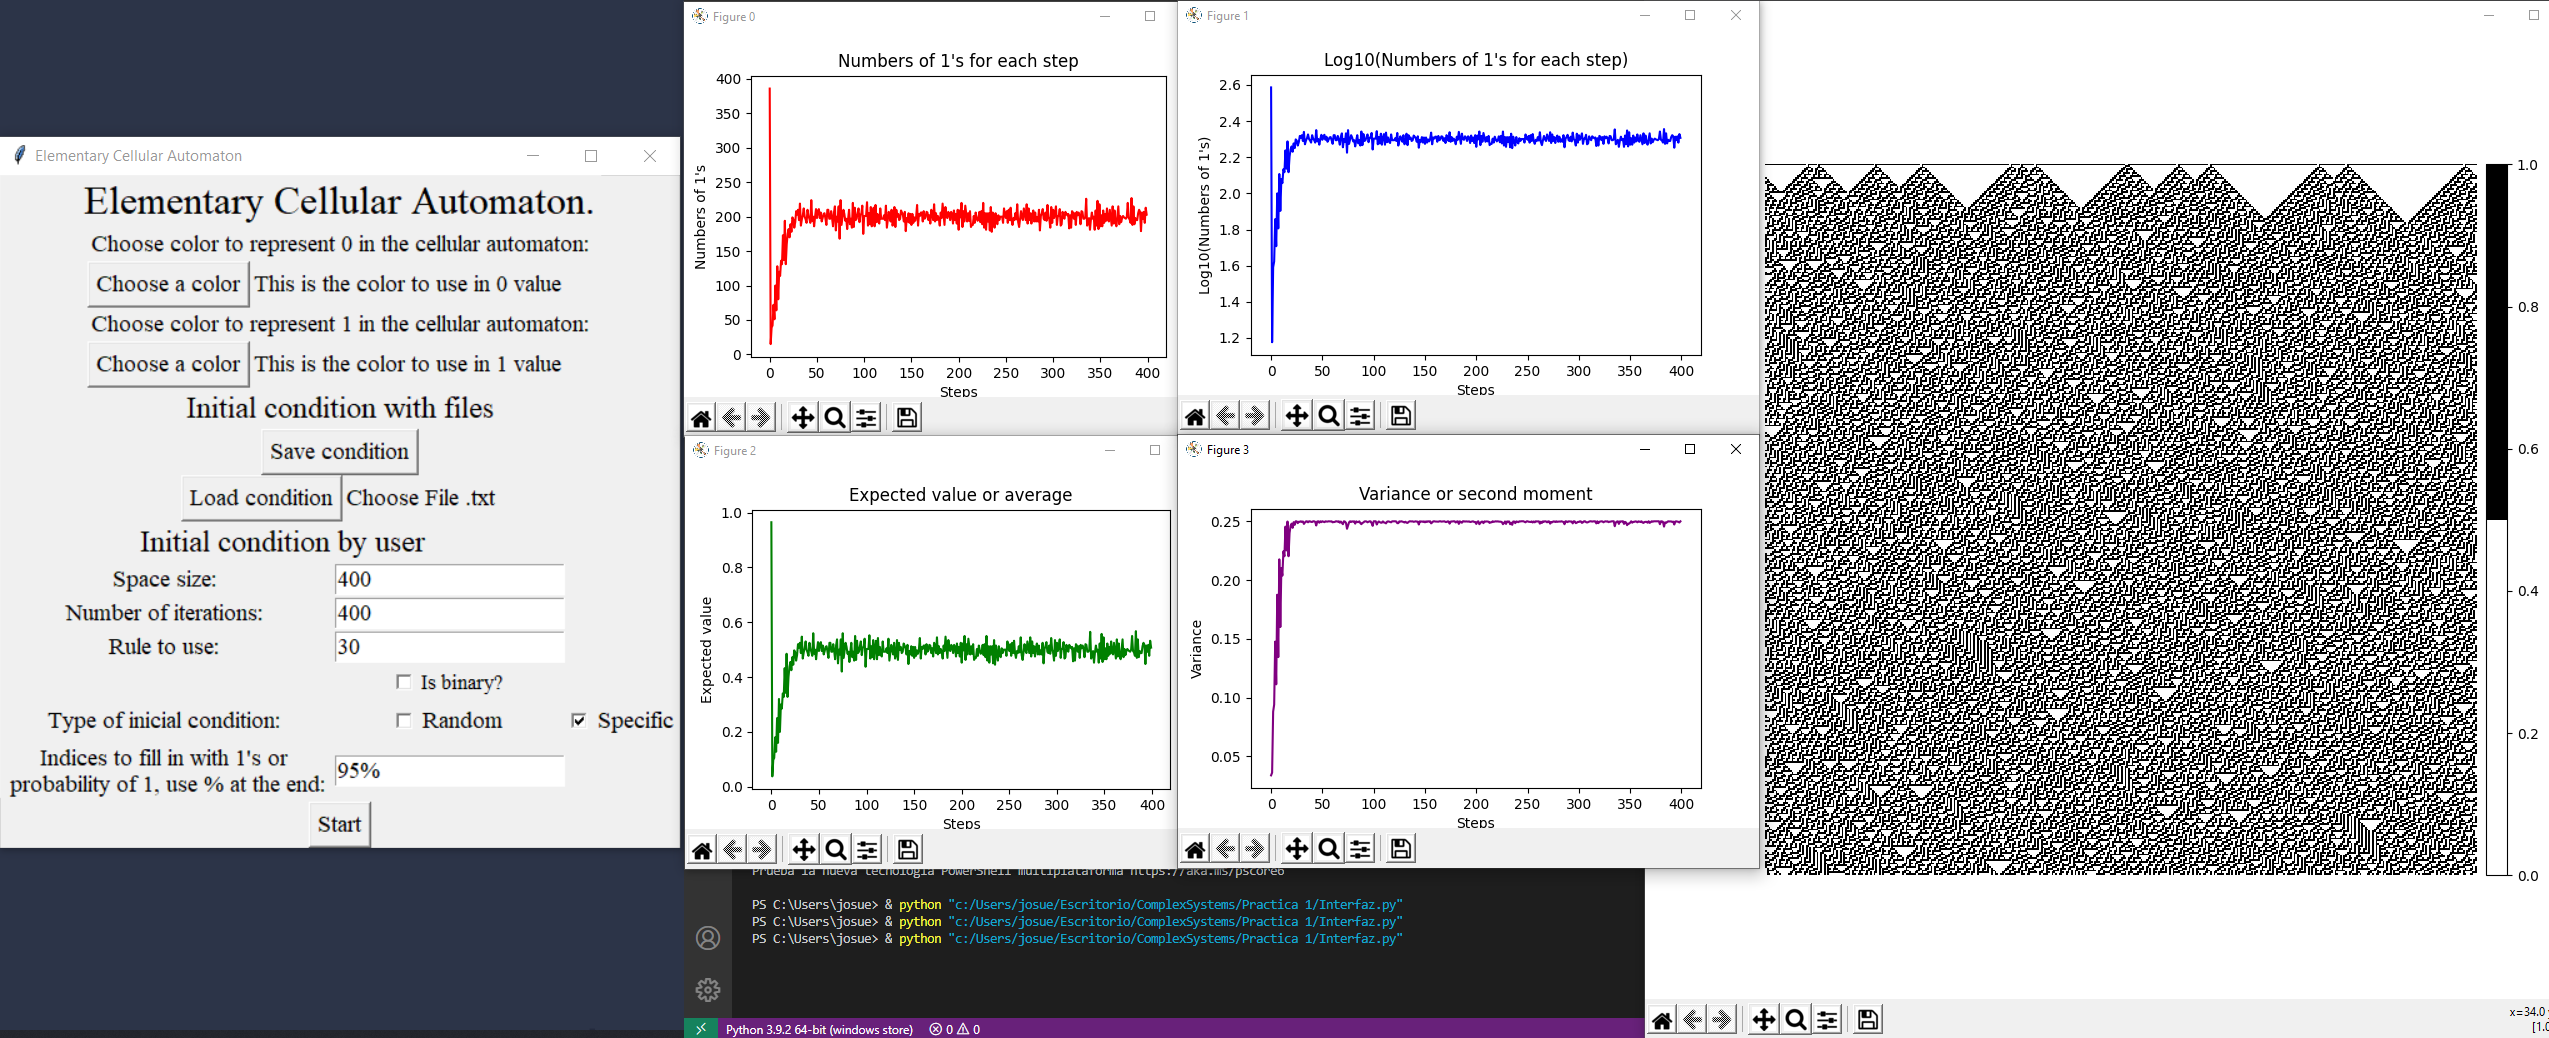
\includegraphics[scale=0.26]{resources/add9.png}
			\caption{ECA de 400 células por 400 iteraciones con 95\% de probabilidad de 1's, regla 30}								\label{fig:picture}
		\end{figure}
		Como vemos en las figuras 18 a la 20 esta regla nos recuerda el comportamiento de la regla anterior, en el sentido de que las figuras 18 y 20 son muy similares en su comportamiento el cual es como un crecimiento logarítmico, en cambio la figura 19 tiene un comportamiento caótico.\par
		Continuando, ahora veremos la regla 54.
		\begin{figure}[H]
			\centering
			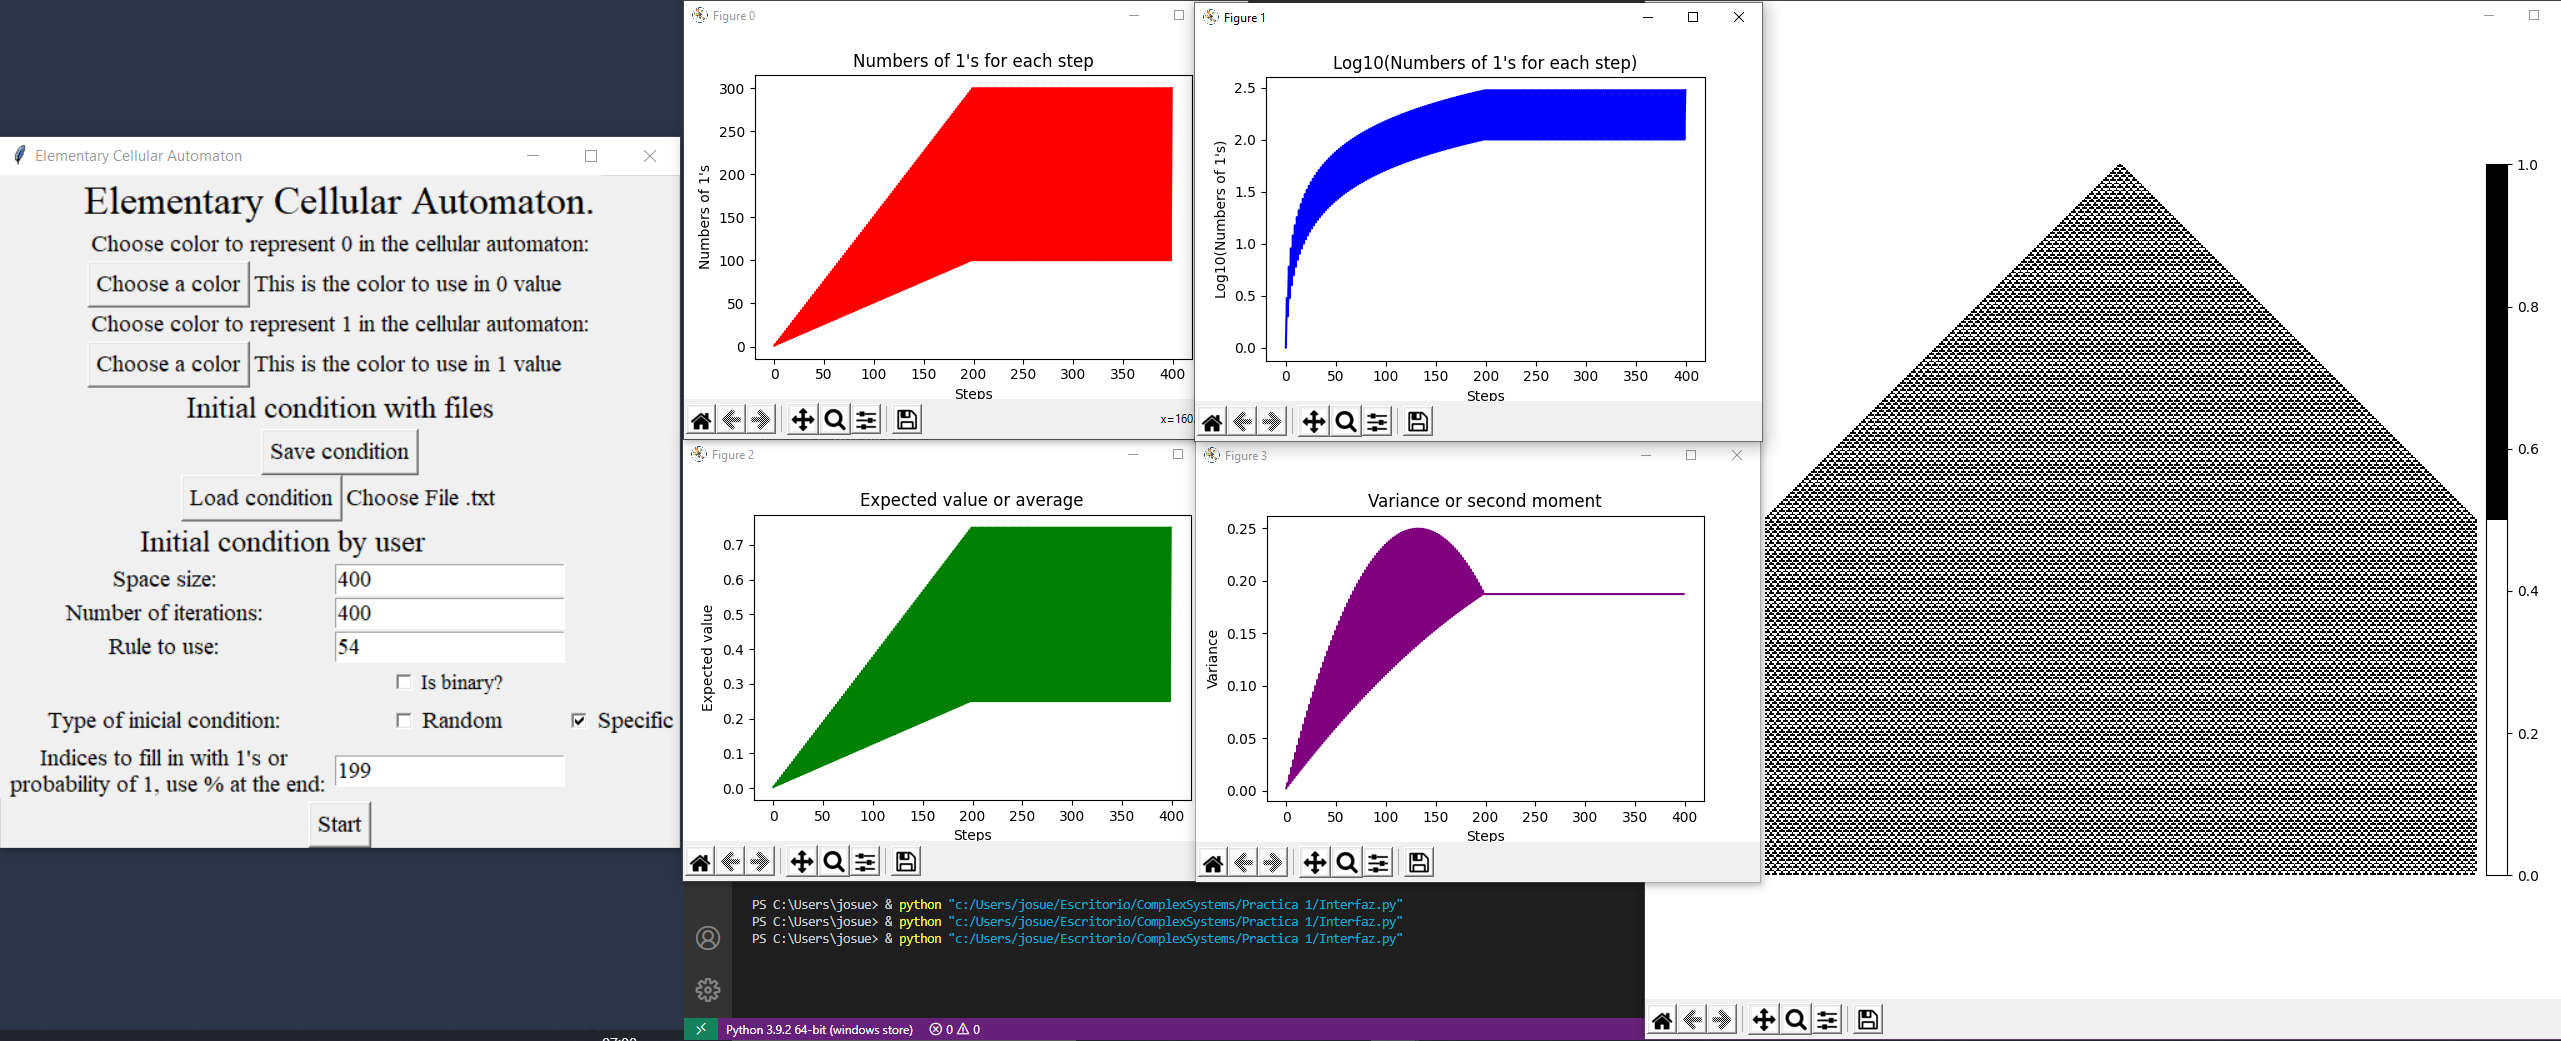
\includegraphics[scale=0.26]{resources/add10.png}
			\caption{ECA de 400 células por 400 iteraciones con una célula inicial central, regla 54}								\label{fig:picture}
		\end{figure}
		\begin{figure}[H]
			\centering
			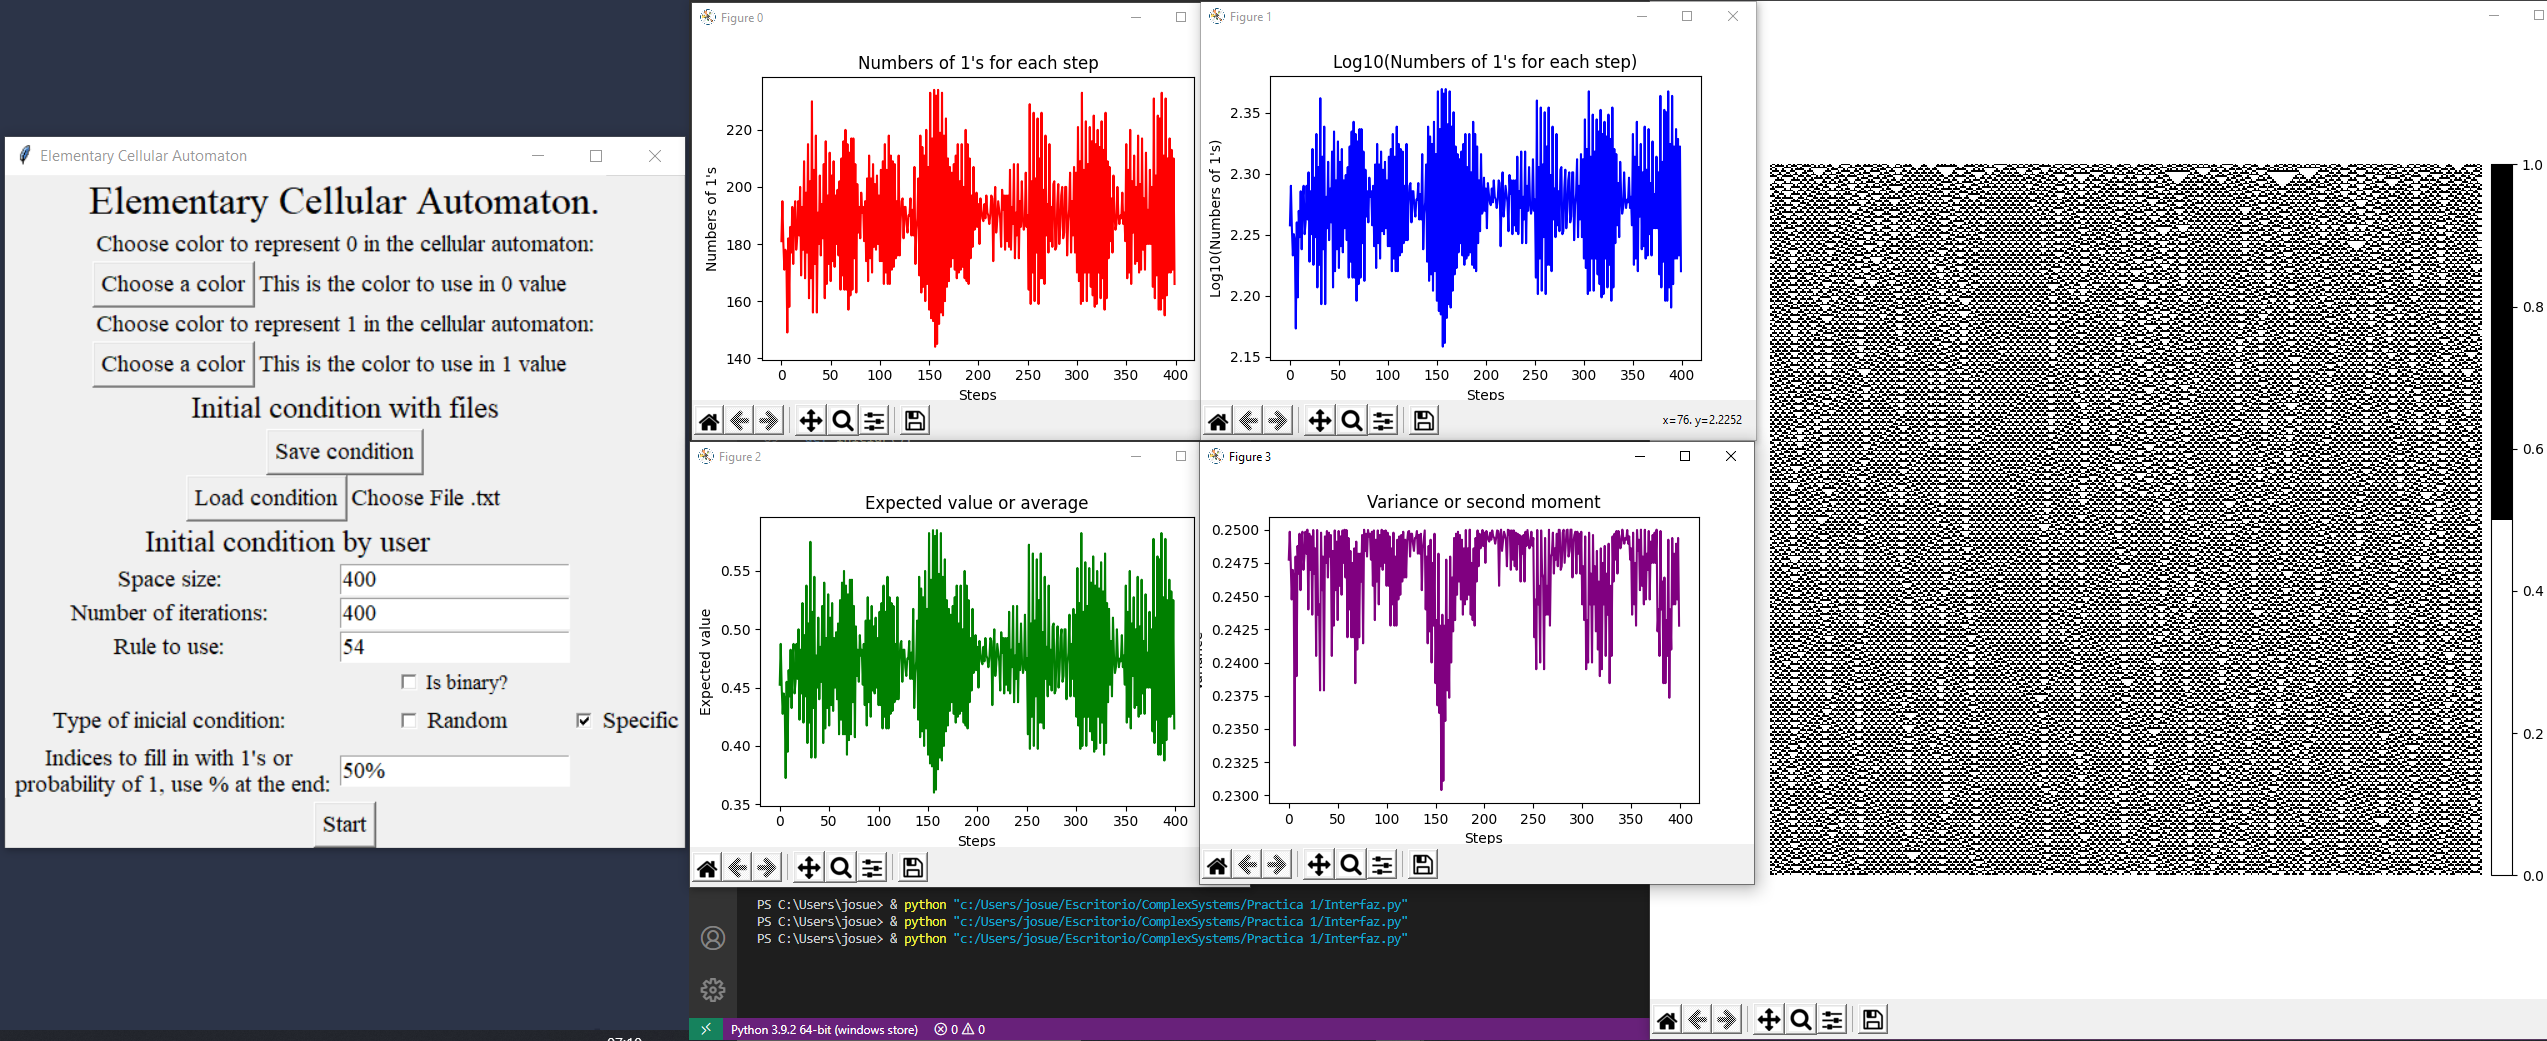
\includegraphics[scale=0.26]{resources/add11.png}
			\caption{ECA de 400 células por 400 iteraciones con 50\% de probabilidad de 1's, regla 54}								\label{fig:picture}
		\end{figure}
		\begin{figure}[H]
			\centering
			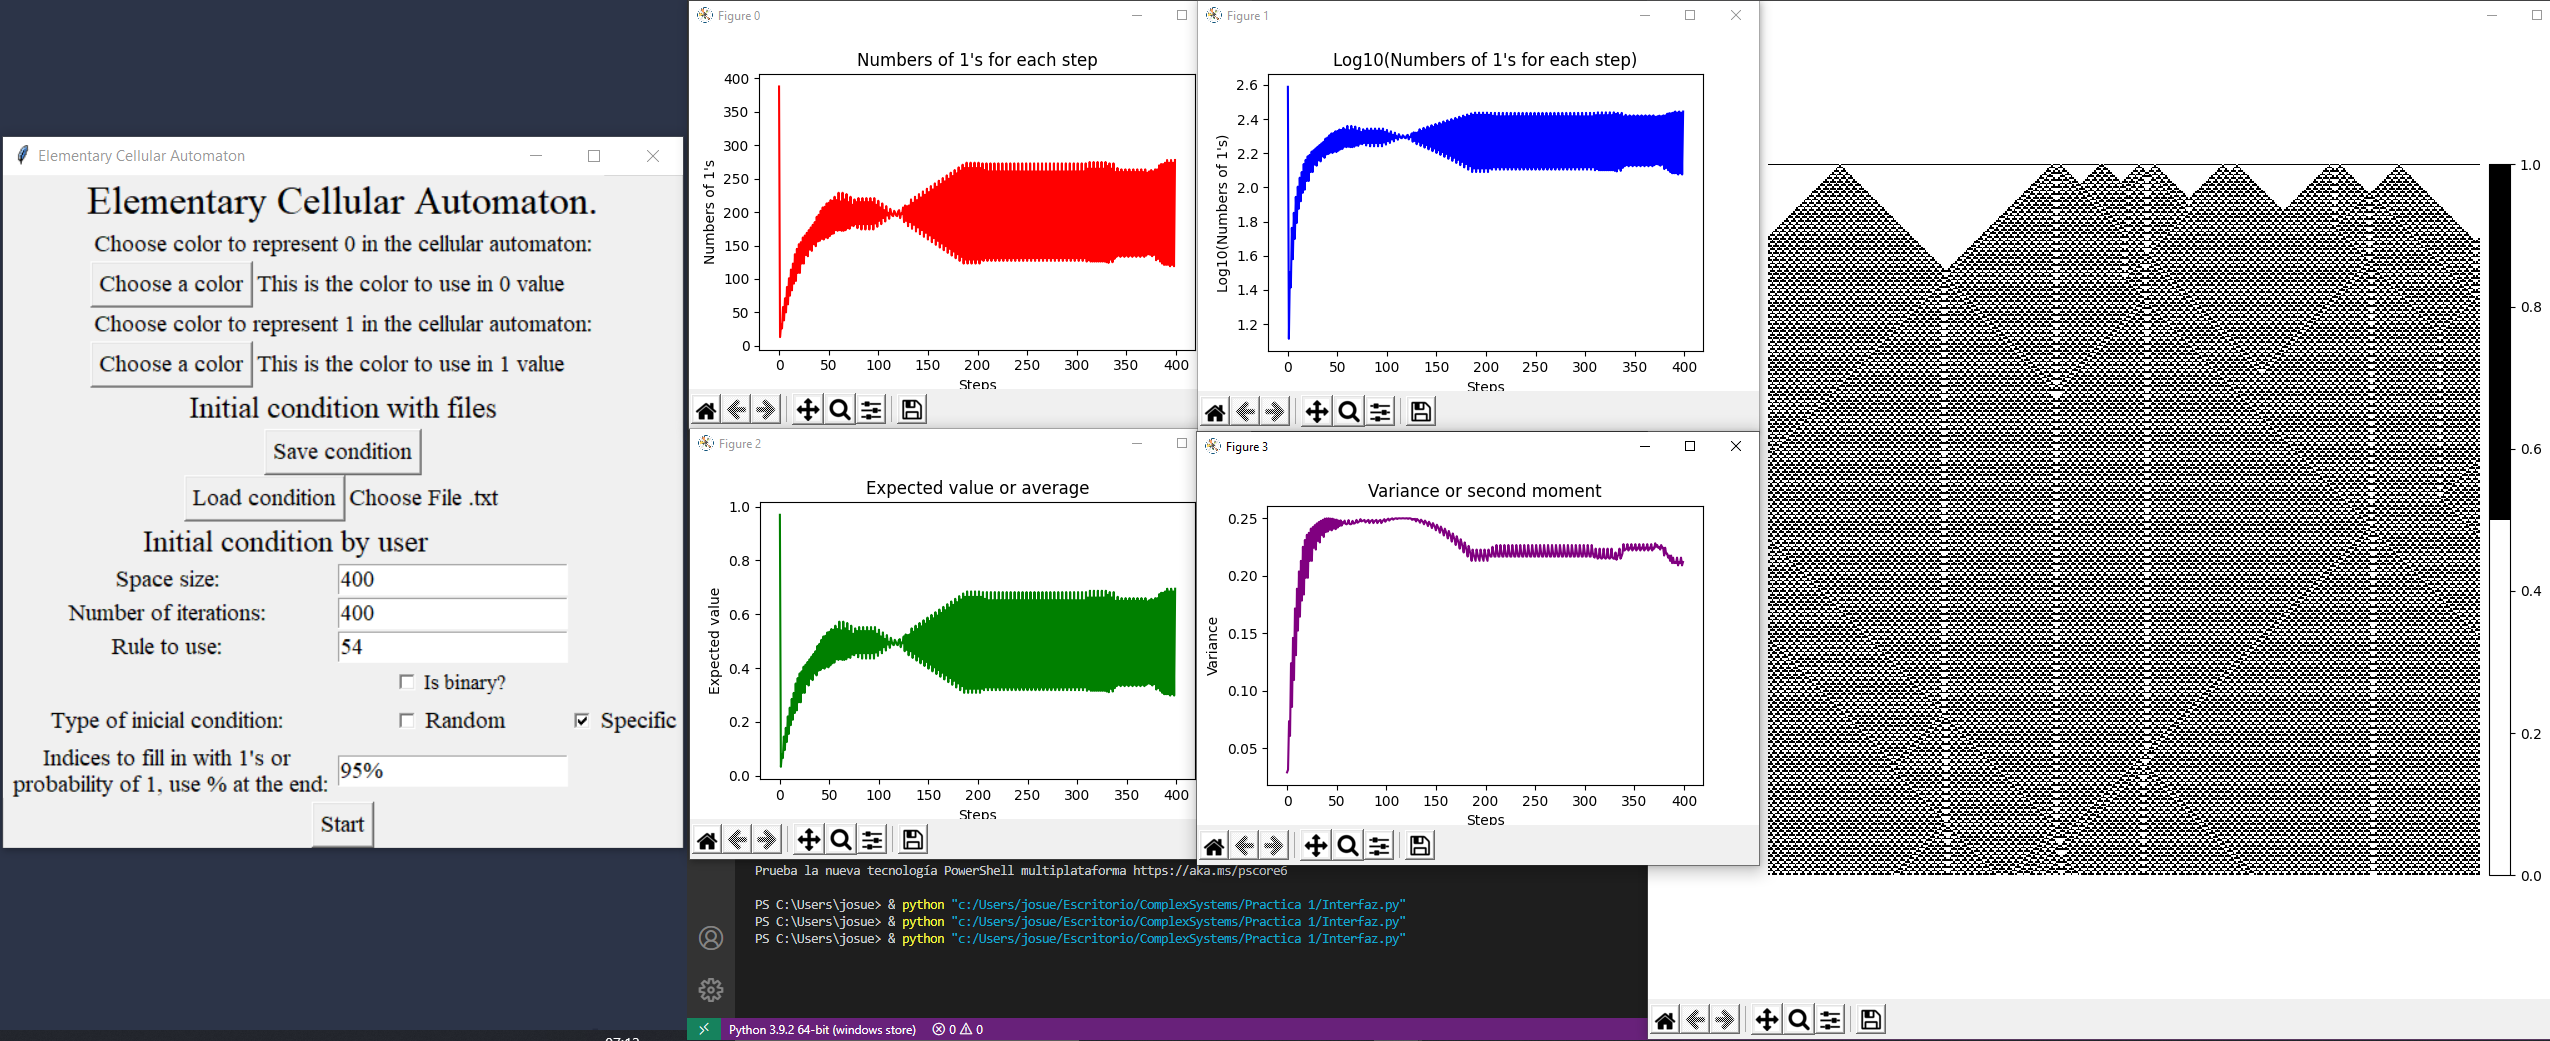
\includegraphics[scale=0.26]{resources/add12.png}
			\caption{ECA de 400 células por 400 iteraciones con 95\% de probabilidad de 1's, regla 54}								\label{fig:picture}
		\end{figure}
		Con esta regla si observamos un cambio en nuestras 3 pruebas que las 3 son diferentes entre si, pero, si observamos la figura 22 y la 23 encontramos una similitud un poco sutil en nuestro ECA y es que ambos generan lineas rectas que $"$dividen$"$ a nuestro ECA de formar vertical, caso contrario a la figura 21 que podríamos decir que esa división pasa a su forma horizontal\par 
		Pasando con la penúltima regla a probar la cual es la regla 110.
		\begin{figure}[H]
			\centering
			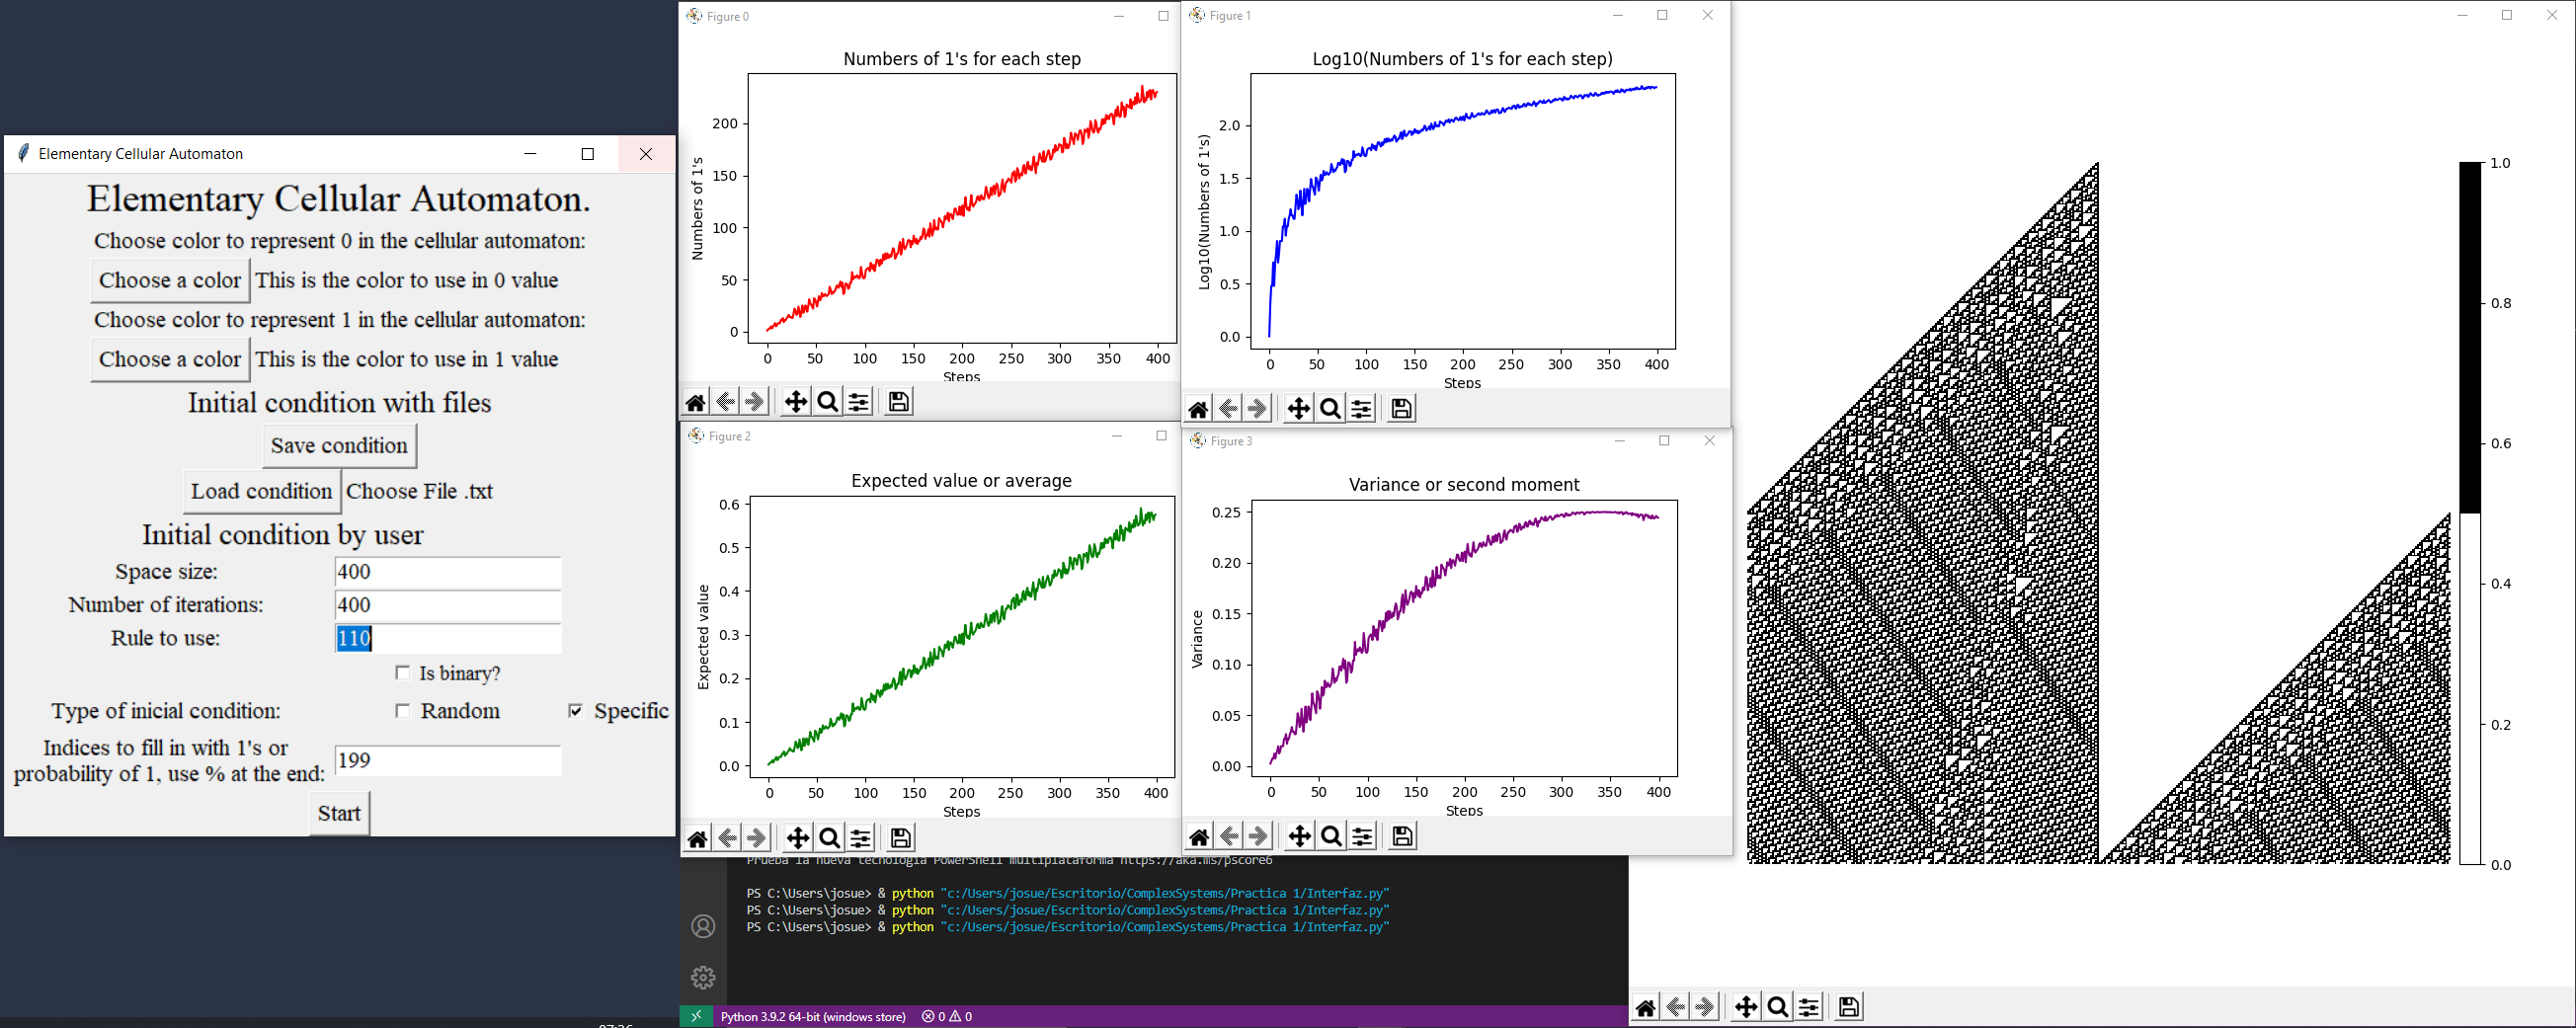
\includegraphics[scale=0.26]{resources/add13.png}
			\caption{ECA de 400 células por 400 iteraciones con una célula inicial central, regla 110}								\label{fig:picture}
		\end{figure}
		\begin{figure}[H]
			\centering
			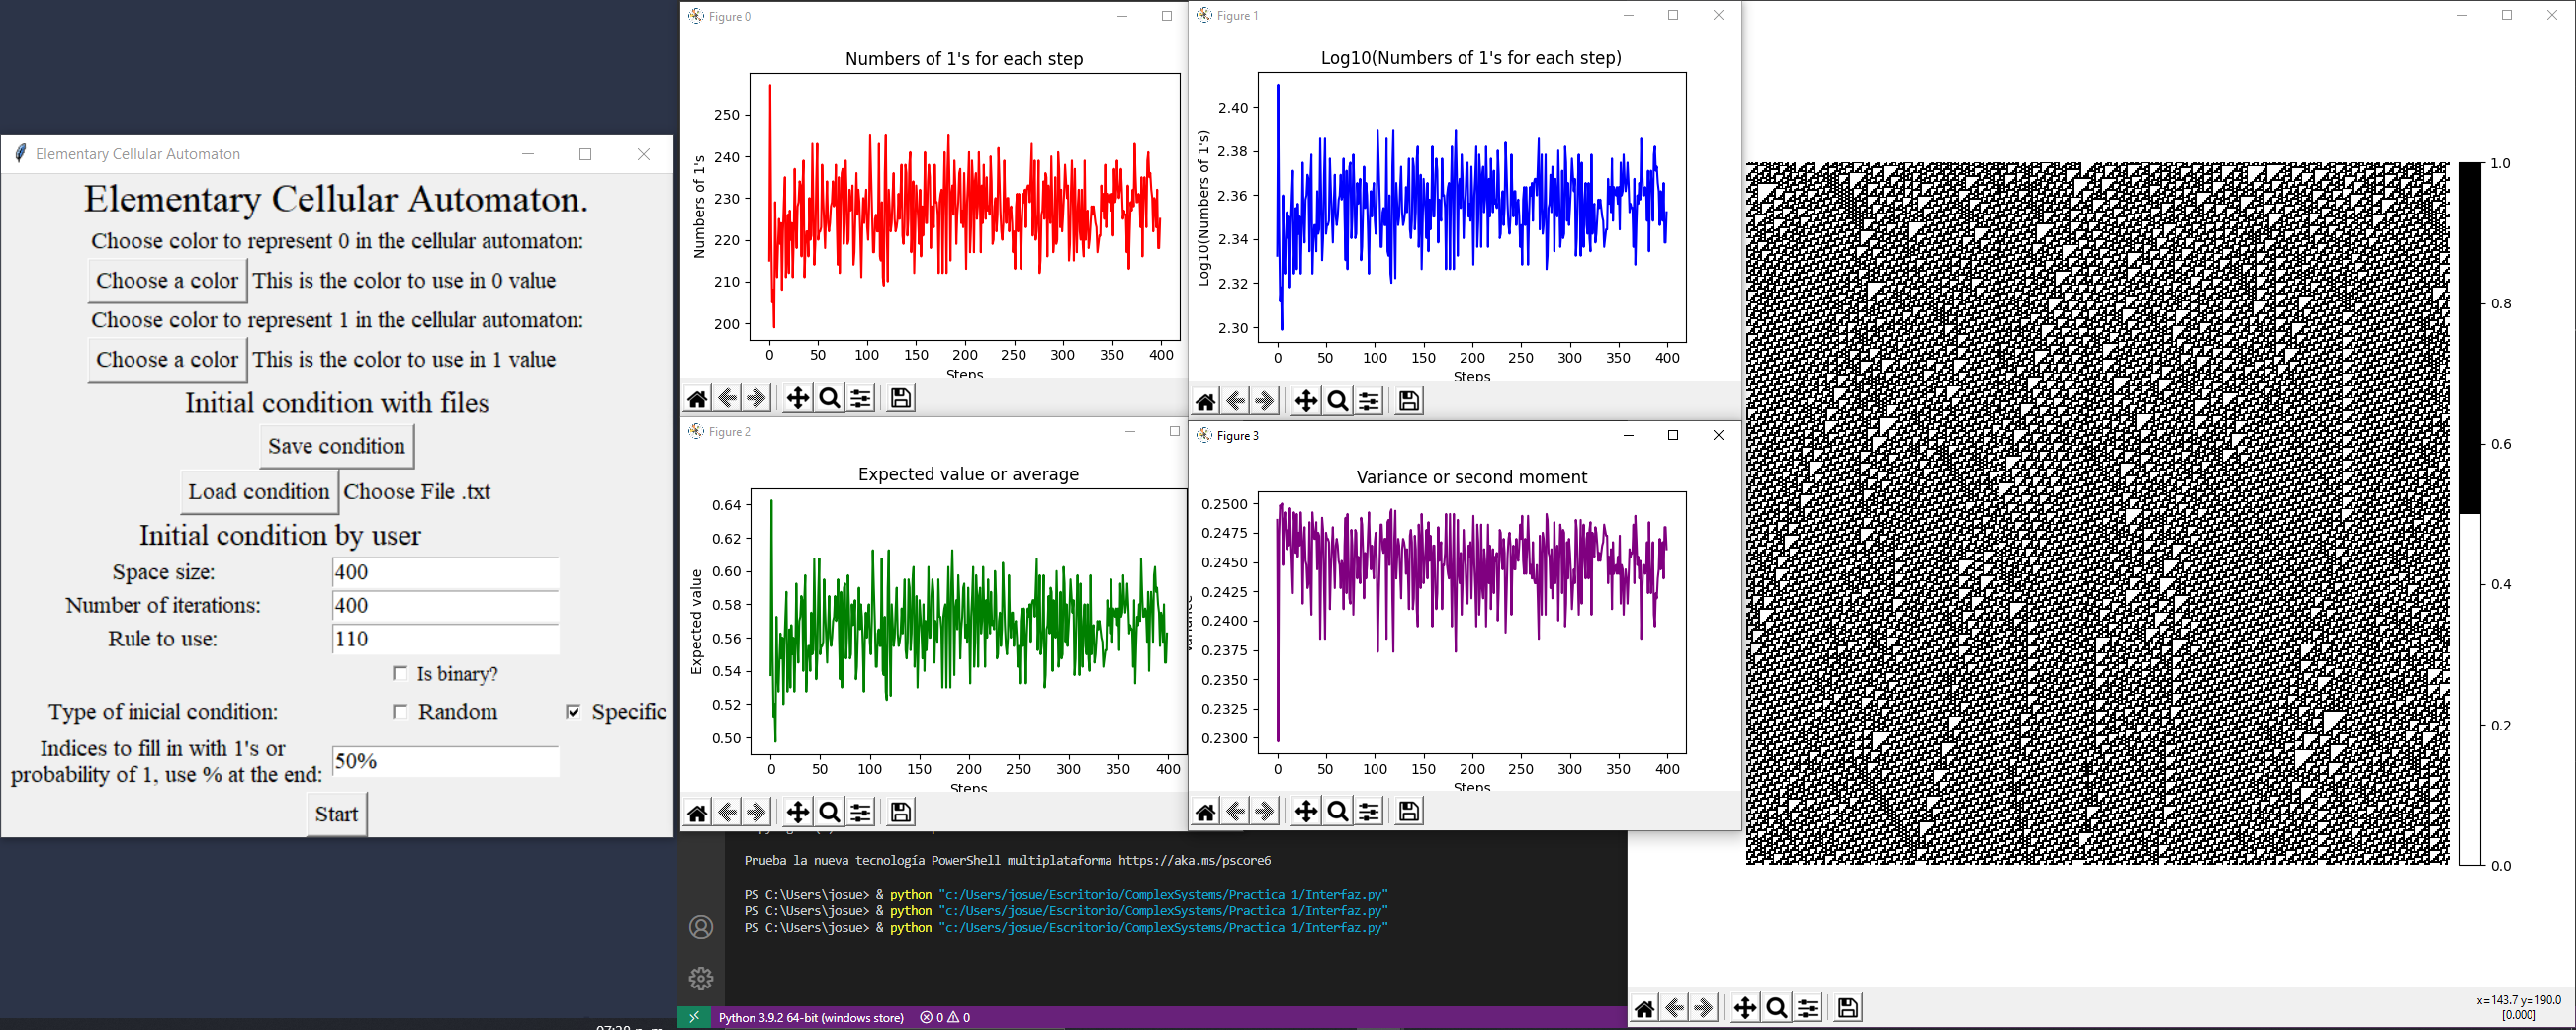
\includegraphics[scale=0.26]{resources/add14.png}
			\caption{ECA de 400 células por 400 iteraciones con 50\% de probabilidad de 1's, regla 110}								\label{fig:picture}
		\end{figure}
		\begin{figure}[H]
			\centering
			\includegraphics[scale=0.26]{resources/add15.png}
			\caption{ECA de 400 células por 400 iteraciones con 95\% de probabilidad de 1's, regla 110}								\label{fig:picture}
		\end{figure}
		Sin duda es la regla con un comportamiento muy interesante, en la figura 24 vemos un crecimiento lineal en los números de células con valor 1, caso contrario de las figuras 25 y 26 las cuales tienen un comportamiento diferente la cual nos recuerda al crecimiento logarítmico, pero, mencionar que la figura 25 no se visualiza tan claramente este comportamiento, de hecho pareciera que estuviéramos algún tipo de filtro en las gráficas de la figura 25 y así obtenemos las gráficas de la figura 26.\par
		Finalmente, tenemos la regla 126.
		\begin{figure}[H]
			\centering
			\includegraphics[scale=0.26]{resources/add16.png}
			\caption{ECA de 400 células por 400 iteraciones con una célula inicial central, regla 126}								\label{fig:picture}
		\end{figure}
		\begin{figure}[H]
			\centering
			\includegraphics[scale=0.26]{resources/add17.png}
			\caption{ECA de 400 células por 400 iteraciones con 50\% de probabilidad de 1's, regla 126}								\label{fig:picture}
		\end{figure}
		\begin{figure}[H]
			\centering
			\includegraphics[scale=0.26]{resources/add18.png}
			\caption{ECA de 400 células por 400 iteraciones con 95\% de probabilidad de 1's, regla 126}								\label{fig:picture}
		\end{figure}
		En el caso de la regla 126 nos recuerda a la regla 22 y es que las imágenes resultantes son muy parecidas, sin embargo, en los casos del 50\% y 95\% vemos como ahora las gráficas son mas definidas en contraste a la regla 22 y que de hecho se parecen a gráficas anteriores en donde mencionamos que se nos recuerda a un crecimiento logarítmico.
		\subsection{Añadidos}
		Como añadidos al programa se agregaron 3 tipos de gráficas, las cuales son las siguientes:
		\begin{itemize}
    		\item Gráfica de logaritmo base 10 de la cantidad de células con valor 1 por cada iteración.
		    \item Gráfica del valor esperado o promedio.
		    \item Gráfica de la varianza o segundo momento.
		\end{itemize}\par		

 		Finalmente para la gráfica de la varianza o segundo momento se usa la siguiente formula para el caso discreto. \[ \sigma^2 =  E[(x-\mu)^2]\] La cual puede ser reducida mediante desarrollo matemático quedando de la siguiente manera: \[ \sigma^2 =  E[(x-\mu)^2] = E[x^2-2x\mu+\mu^2]\]        \[ \sigma^2 = E[x^2]-E[2x\mu]+E[\mu^2]\]	\[ \sigma^2 = E[x^2]-2\mu E[x]+\mu^2\]						\[ \sigma^2 = E[x^2]-2\mu\mu+\mu^2\]	\[ \sigma^2 = E[x^2]-2\mu^2+\mu^2\] Finalmente tenemos que: 	\[ \sigma^2 = E[x^2]-\mu^2\]
 		Por lo que, retomando lo mencionado para el desarrollo de la gráfica 2 o la gráfica de nuestro promedio o valor esperado solo necesitamos el valor de $f(x=1)$, nuestra nuestra formula para la varianza y finalmente saber que $E[x^n] =  \sum_{x} x^n *f(x) $, así, sustituyendo valores obtendríamos lo siguiente sera: \[ \sigma^2 = (1^2*f(x=1)) - f(x=1)^2 = f(x=1) - f(x=1)^2 \] Finalmente la formula a usar para la varianza: \[ \sigma^2 = f(x=1) - f(x=1)^2 \]
 		Ahora hagamos una prueba, en la cual la regla a usar sera la regla 30, un tamaño de 1000 células con 1000 iteraciones, colores por defecto y asignación de células con valor 1 de manera aleatoria.
 		\begin{figure}[H]
			\centering
			\includegraphics[scale=0.35]{resources/pruebaF1.png}
			\caption{ECA de 1000 células por 1000 iteraciones creado de forma aleatoria}\label{fig:picture}
		\end{figure}
		Como podemos observar tenemos 3 graficas que tienen una forma similar o casi iguales las cuales son la cantidad de 1's por iteración, $log$ de la cantidad de 1's y el valor esperado, esto es lógico ya que solo estamos cambiando la $"$escala$"$ de una misma representación, la única gráfica que difiere de las demás es la varianza y esto resulta, como dato adicional al momento de usar diferentes reglas el comportamiento de esta difiere e incluso en ocasiones llega a ser similar con las otras 3. Como nota adicional mencionar que a cada gráfica le podemos incrementar el tamaño de la gráfica para poder visualizar de una mejor visualización de los datos, lo anterior se realiza exactamente igual que a como se menciono unas hojas atrás.\par
		Adicionalmente a lo anterior, la barra de opciones que tiene cada gráfica nos permite realizar diferentes cosas que en seguida enlistaremos, para comodidad tomar como referencia la figura 12 y ver los iconos de izquierda a derecha.
		\begin{enumerate}
		  \item El icono de la casa nos permite reajustar la vista de nuestra gráfica a como lo era originalmente.
		  \item El icono de la flecha a la izquierda o derecha nos permite navegar entre las distintas vistas que hayamos realizado en una gráfica, es decir, si hicimos dos aumentos y queremos regresar al primero hacemos de la flecha hacia la izquierda y en caso de que estando en el primer aumento queremos regresar al segundo hacemos uso de la flecha a la derecha.
		  \item El icono que nos recuerda a una cruz nos permite mover la gráfica a voluntad, un ejemplo de uso seria que al hacer zoom en un área y querer mover ese mismo zoom en un área que tenemos a lado hacemos uso de esta función para poder mover nuestra gráfica.
		  \item El icono de la lupa como ya se ha mencionado nos permite aumentar el tamaño de cierta área en nuestra gráfica.
		  \item El icono que nos recuerda a configuración no recomiendo usarlo ya que cambia la configuración inicial de nuestra gráfica y en ocasiones nos arruina el como se ve la gráfica
		  \item El ultimo icono, que es el icono de disquete nos permite, como es incluso lógico, guardar la gráfica como una imagen con varias extensiones a elegir, esto nos permite poder guardar resultados como una imagen para el posterior uso.
		\end{enumerate}
		\begin{figure}[H]
			\centering
			\includegraphics[scale=1]{resources/barra.png}
			\caption{Barra de opciones}\label{fig:picture}
		\end{figure}
		\newpage
		\subsection{Código}
	A continuación se anexa el código generado para la creación de este primer programa. Primero
tenemos la parte de la interfaz de nuestro programa que se crea con el siguiente código.
\par
	Por ultimo tenemos el código que nos proporciona la parte lógica del programa y que ademas es el encargado de hacer las gráficas, este código es el cerebro de nuestro programa.

	\section{Conclusiones}
	Esta programa es bastante interesante, ya que es increíble ver al cambiar los valores de las células de nuestra iteración cero cambia por mucho el comportamiento de nuestro ECA que se podria pensar que no es tan significativo pero eso es un pensamiento errado ya que vemos 	que cambia demasiado, podríamos llegar a decir que una célula de mas o de menos provoca un caos en nuestro ECA y por tanto un ECA diferente cada vez que cambiemos nuestra iteración inicial. Finalmente solo me queda comentar que al haber ya probado diferentes reglas con la misma iteración inicial el resultado es muy diferente con cada regla.
	\begin{thebibliography}{1}
 \bibitem[label1]{cite_key1} Weisstein, E., 2021. Elementary Cellular Automaton - from Wolfram MathWorld. [online] Mathworld.wolfram.com. Available at: https://mathworld.wolfram.com/ElementaryCellularAutomaton.html [Accessed 15 March 2021].	
 \bibitem[label2]{cite_key2} Lees, E., 2020. Elementary Cellular Automata · Matplotblog. [online] Matplotlib.org. Available at: https://matplotlib.org/matplotblog/posts/elementary-cellular-automata/ [Accessed 15 March 2021].
  \bibitem[label3]{cite_key3} Caparrini, F., 2016. Autómatas Celulares - Fernando Sancho Caparrini. [online] Cs.us.es. Available at: \url{http://www.cs.us.es/~fsancho/?e=66} [Accessed 15 March 2021].
\end{thebibliography}

\end{document}
